\documentclass[12pt]{article}
\usepackage[margin=1in]{geometry}
\usepackage{booktabs}
\usepackage{longtable}
\usepackage{caption}
\usepackage{graphicx}
\usepackage{float}
\DeclareCaptionLabelSeparator{emdash}{---}
\captionsetup{font=normalsize,labelfont=sc,textfont=sc,labelsep=emdash}
\captionsetup[figure]{position=top,justification=centering}
\def\sym#1{\ifmmode^{#1}\else\(^{#1}\)\fi}
\graphicspath{{../Output/Figures/Main/}{Output/Figures/Main/}{./}}
\title{Results First Draft}
\author{Zachary Serby}
\date{\today}
\begin{document}
\maketitle
\thispagestyle{empty}
\clearpage

\subsection*{Summary Statistics}

\begingroup
\footnotesize
\renewcommand{\arraystretch}{0.86}
\setlength{\tabcolsep}{4pt}
\setlength{\LTcapwidth}{\textwidth}
\begin{longtable}{l*{6}{c}}
\caption{Summary Statistics, 2009 Drought DID Samples}\\
\toprule
 & \multicolumn{6}{c}{Panel A: WAZ, age \ensuremath{\le}10 in 2005 and 2009}\\
\cmidrule(lr){2-7}
                    &        Mean&   Std. dev.&        Min.&      Median&        Max.&        Obs.\\
\midrule
\textit{Outcomes (MxFLS-2, 2005)}&            &            &            &            &            &            \\
Weight-for-age z-score (WAZ)&       -0.32&        1.41&       -5.07&       -0.37&        4.51&       1,084\\
\addlinespace[6pt]\textit{Binary DID treatment (CHIRPS)}&            &            &            &            &            &            \\
2009 drought (indicator)&        0.39&        0.49&        0.00&        0.00&        1.00&       1,084\\
2005 drought (indicator)&        0.64&        0.48&        0.00&        1.00&        1.00&       1,084\\
2006 drought (indicator)&        0.06&        0.24&        0.00&        0.00&        1.00&       1,084\\
2007 drought (indicator)&        0.19&        0.40&        0.00&        0.00&        1.00&       1,084\\
2008 drought (indicator)&        0.19&        0.39&        0.00&        0.00&        1.00&       1,084\\
\addlinespace[6pt]\textit{Continuous DID treatment (CHIRPS)}&            &            &            &            &            &            \\
2009 rainfall deficit (SD)&        0.76&        0.72&        0.00&        0.55&        2.51&       1,084\\
Any 2009 rainfall deficit (indicator)&        0.77&        0.42&        0.00&        1.00&        1.00&       1,084\\
\addlinespace[6pt]\textit{Remittances (MxFLS-1, 2002)}&            &            &            &            &            &            \\
Household received remittances, proxy (indicator)&        0.40&        0.49&        0.00&        0.00&        1.00&         725\\
\addlinespace[6pt]\textit{Household (MxFLS-1, 2002)}&            &            &            &            &            &            \\
Dwelling has electricity (indicator)&        0.98&        0.15&        0.00&        1.00&        1.00&         818\\
Good floor quality (indicator)&        0.83&        0.37&        0.00&        1.00&        1.00&         818\\
Good roof quality (indicator)&        0.82&        0.38&        0.00&        1.00&        1.00&         818\\
Enough ventilation (indicator)&        0.56&        0.50&        0.00&        1.00&        1.00&         812\\
Sleeping rooms per household member&        0.41&        0.24&        0.11&        0.33&        2.33&         817\\
Ln (monthly expenditure per capita, pesos), proxy&        6.56&        0.86&        4.21&        6.57&       11.43&         803\\
Rural locality (indicator)&        0.43&        0.50&        0.00&        0.00&        1.00&         818\\
\addlinespace[6pt]\textit{Child and mother (MxFLS-2, 2005)}&            &            &            &            &            &            \\
Age (years, not in regression)&        2.43&        1.69&        0.00&        2.00&        6.00&       1,084\\
Male (indicator)    &        0.51&        0.50&        0.00&        1.00&        1.00&       1,084\\
Fully vaccinated (indicator)&        0.36&        0.48&        0.00&        0.00&        1.00&       1,029\\
Mother's height (centimeters)&      154.69&        6.85&      136.00&      154.50&      182.70&       1,033\\
Mother's years of schooling&        7.53&        3.42&        0.00&        8.00&       18.00&       1,047\\
Mother's age at birth (years)&       26.00&        6.49&       12.00&       25.00&       59.00&       1,055\\
Mother employed (indicator)&        0.24&        0.42&        0.00&        0.00&        1.00&       1,046\\
\addlinespace[6pt]\textit{Father and birth (MxFLS-1 and MxFLS-2)}&            &            &            &            &            &            \\
Father's height (centimeters)&      166.73&        7.16&      144.00&      166.70&      192.00&         713\\
Father's years of schooling&        7.72&        3.64&        0.00&        9.00&       18.00&         872\\
Father's age at birth (years)&       29.44&        7.74&       13.00&       28.00&       75.00&         895\\
Father employed (indicator)&        0.96&        0.20&        0.00&        1.00&        1.00&         872\\
Birth order         &        2.07&        1.58&        1.00&        2.00&       13.00&         617\\
Oldest child (indicator)&        0.48&        0.50&        0.00&        0.00&        1.00&         617\\
Birth weight (kilograms)&        3.24&        0.56&        1.55&        3.20&        5.50&         767\\
Delivered at home (indicator)&        0.07&        0.26&        0.00&        0.00&        1.00&         818\\
Weeks predominantly breastfed&       32.07&       29.15&        0.00&       26.09&      206.00&         790\\
Iron during pregnancy (indicator)&        0.78&        0.41&        0.00&        1.00&        1.00&         799\\
Premature, mother reported (indicator)&        0.18&        0.38&        0.00&        0.00&        1.00&         796\\

\bottomrule
\newpage
\toprule
 & \multicolumn{6}{c}{Panel B: HAZ and BMIZ, age \ensuremath{\le}15 in 2005 and 2009}\\
\cmidrule(lr){2-7}
                    &        Mean&   Std. dev.&        Min.&      Median&        Max.&        Obs.\\
\midrule
\textit{Outcomes (MxFLS-2, 2005)}&            &            &            &            &            &            \\
Height-for-age z-score (HAZ)&       -0.60&        1.48&       -5.46&       -0.64&        5.65&       2,436\\
BMI-for-age z-score (BMIZ)&        0.36&        1.43&       -4.95&        0.30&        4.97&       2,393\\
\addlinespace[6pt]\textit{Binary DID treatment (CHIRPS)}&            &            &            &            &            &            \\
2009 drought (indicator)&        0.41&        0.49&        0.00&        0.00&        1.00&       2,436\\
2005 drought (indicator)&        0.62&        0.49&        0.00&        1.00&        1.00&       2,436\\
2006 drought (indicator)&        0.07&        0.25&        0.00&        0.00&        1.00&       2,436\\
2007 drought (indicator)&        0.20&        0.40&        0.00&        0.00&        1.00&       2,436\\
2008 drought (indicator)&        0.19&        0.39&        0.00&        0.00&        1.00&       2,436\\
\addlinespace[6pt]\textit{Continuous DID treatment (CHIRPS)}&            &            &            &            &            &            \\
2009 rainfall deficit (SD)&        0.79&        0.73&        0.00&        0.60&        2.51&       2,436\\
Any 2009 rainfall deficit (indicator)&        0.79&        0.41&        0.00&        1.00&        1.00&       2,436\\
\addlinespace[6pt]\textit{Remittances (MxFLS-1, 2002)}&            &            &            &            &            &            \\
Household received remittances, proxy (indicator)&        0.36&        0.48&        0.00&        0.00&        1.00&       1,849\\
\addlinespace[6pt]\textit{Household (MxFLS-1, 2002)}&            &            &            &            &            &            \\
Dwelling has electricity (indicator)&        0.98&        0.15&        0.00&        1.00&        1.00&       2,035\\
Good floor quality (indicator)&        0.83&        0.38&        0.00&        1.00&        1.00&       2,035\\
Good roof quality (indicator)&        0.81&        0.39&        0.00&        1.00&        1.00&       2,035\\
Enough ventilation (indicator)&        0.56&        0.50&        0.00&        1.00&        1.00&       2,020\\
Sleeping rooms per household member&        0.38&        0.22&        0.10&        0.33&        2.33&       2,032\\
Ln (monthly expenditure per capita, pesos), proxy&        6.51&        0.85&        3.75&        6.51&       12.24&       2,005\\
Rural locality (indicator)&        0.45&        0.50&        0.00&        0.00&        1.00&       2,035\\
\addlinespace[6pt]\textit{Child and mother (MxFLS-2, 2005)}&            &            &            &            &            &            \\
Age (years, not in regression)&        5.86&        3.29&        0.00&        6.00&       15.00&       2,436\\
Male (indicator)    &        0.50&        0.50&        0.00&        0.00&        1.00&       2,436\\
Fully vaccinated (indicator)&        0.48&        0.50&        0.00&        0.00&        1.00&       2,314\\
Mother's height (centimeters)&      154.30&        6.99&      133.40&      154.10&      190.00&       2,300\\
Mother's years of schooling&        7.17&        3.67&        0.00&        7.00&       18.00&       2,328\\
Mother's age at birth (years)&       26.41&        6.53&       12.00&       26.00&       59.00&       2,354\\
Mother employed (indicator)&        0.29&        0.45&        0.00&        0.00&        1.00&       2,329\\
\addlinespace[6pt]\textit{Father and birth (MxFLS-1 and MxFLS-2)}&            &            &            &            &            &            \\
Father's height (centimeters)&      166.38&        7.13&      144.00&      166.20&      192.00&       1,619\\
Father's years of schooling&        7.40&        3.87&        0.00&        8.00&       18.00&       1,934\\
Father's age at birth (years)&       29.83&        7.84&       13.00&       29.00&       75.00&       2,004\\
Father employed (indicator)&        0.96&        0.20&        0.00&        1.00&        1.00&       1,938\\
Birth order         &        2.55&        1.88&        1.00&        2.00&       13.00&       1,734\\
Oldest child (indicator)&        0.36&        0.48&        0.00&        0.00&        1.00&       1,734\\
Birth weight (kilograms)&        3.25&        0.59&        0.85&        3.20&        6.00&       1,589\\
Delivered at home (indicator)&        0.11&        0.32&        0.00&        0.00&        1.00&       1,924\\
Weeks predominantly breastfed&       33.48&       33.28&        0.00&       26.09&      260.89&       1,706\\
Iron during pregnancy (indicator)&        0.73&        0.44&        0.00&        1.00&        1.00&       1,718\\
Premature, mother reported (indicator)&        0.14&        0.34&        0.00&        0.00&        1.00&       1,714\\

\bottomrule
\addlinespace[6pt]\multicolumn{7}{p{0.97\textwidth}}{\scriptsize \textit{Notes:} Sample is children with the outcome measured in MxFLS-2 (2005) and MxFLS-3 (2009), aged 10 or younger (Panel A) or 15 or younger (Panel B)
in both rounds, with a 2005 municipality and not measured in MxFLS-3 before November 2009. Each row is a child, and Obs. counts children. Statistics are at the 2005 baseline, except
remittances and household variables (2002). Panel B reports BMIZ for the HAZ sample, as the BMIZ sample is similar and slightly smaller, at 2,383 children.
The continuous DID uses these samples, and binary DID Model 1 excludes 6 (Panel A) and 4 (Panel B) children in singleton
interview-month cells. Model 3, the main binary DID, adds 2005--2008 droughts and 2002 household and 2005 child and mother controls and includes
700 (WAZ), 1,755 (HAZ), and 1,714 (BMIZ) children. The SPI analysis compares z of -1 or below with z between -1 and 1, excluding
9 (Panel A) and 36 (Panel B) children with z of 1 or above. Drought is annual CHIRPS rainfall in the 2005 municipality below its 1981--2004 20th percentile.
Rainfall deficit is max(0,~-z), where z is 2009 rainfall in standard deviations from the 1981--2004 municipal mean. Remittances, a proxy, are cash received in the last
12 months from parents, siblings, or children outside the household. Expenditure is in 2002 pesos per person per month, a proxy for
household income. Rural is a locality under 2,500 inhabitants (INEGI, 2024).}\\
\end{longtable}
\endgroup
\clearpage
\begingroup
\footnotesize
\renewcommand{\arraystretch}{0.86}
\setlength{\tabcolsep}{4pt}
\setlength{\LTcapwidth}{\textwidth}
\setlength{\LTleft}{0pt}
\setlength{\LTright}{0pt plus 1fil}
\begin{longtable}{@{\extracolsep{\fill}}lcc}
\caption{Sample Sizes, Treated and Control Children}\\
\toprule
 & \multicolumn{2}{c}{Panel A: Binary DID, 2009 drought}\\*
\cmidrule(lr){2-3}
 & Control & Treated\\*
\midrule
\textit{HAZ sample, children aged 15 or younger in 2005 and 2009} & & \\*
Children, estimation sample & 1,442 & 994\\*
Children, Model 1 (basic DID) & 1,439 & 993\\*
Children, Model 3 (DID with controls) & 1,021 & 734\\*
Children, Model 5 (triple difference) & 946 & 676\\*
\quad In 2002 remittance households & 377 & 206\\*
Households, estimation sample & 894 & 628\\*
2005 municipalities, estimation sample & 80 & 53\\
\addlinespace[6pt]\textit{WAZ sample, children aged 10 or younger in 2005 and 2009} & & \\*
Children, estimation sample & 662 & 422\\*
Children, Model 1 (basic DID) & 658 & 420\\*
Children, Model 3 (DID with controls) & 422 & 278\\*
Children, Model 5 (triple difference) & 385 & 249\\*
\quad In 2002 remittance households & 160 & 98\\*
Households, estimation sample & 537 & 344\\*
2005 municipalities, estimation sample & 74 & 49\\
\addlinespace[6pt]\textit{BMIZ sample, children aged 15 or younger in 2005 and 2009} & & \\*
Children, estimation sample & 1,415 & 968\\*
Children, Model 1 (basic DID) & 1,412 & 967\\*
Children, Model 3 (DID with controls) & 1,000 & 714\\*
Children, Model 5 (triple difference) & 926 & 661\\*
\quad In 2002 remittance households & 369 & 201\\*
Households, estimation sample & 881 & 611\\*
2005 municipalities, estimation sample & 80 & 53\\
\bottomrule
\addlinespace[12pt]
\toprule
 & \multicolumn{2}{c}{Panel B: Continuous DID, any 2009 deficit}\\*
\cmidrule(lr){2-3}
 & Control & Treated\\*
\midrule
\textit{HAZ sample, children aged 15 or younger in 2005 and 2009} & & \\*
Children, continuous DID sample & 518 & 1,918\\*
\quad In 2002 remittance households & 111 & 563\\*
\quad In 2002 non-remittance households & 314 & 861\\*
Households & 324 & 1,198\\*
2005 municipalities & 34 & 99\\
\addlinespace[6pt]\textit{WAZ sample, children aged 10 or younger in 2005 and 2009} & & \\*
Children, continuous DID sample & 245 & 839\\*
\quad In 2002 remittance households & 49 & 244\\*
\quad In 2002 non-remittance households & 128 & 304\\*
Households & 200 & 681\\*
2005 municipalities & 30 & 93\\
\addlinespace[6pt]\textit{BMIZ sample, children aged 15 or younger in 2005 and 2009} & & \\*
Children, continuous DID sample & 507 & 1,876\\*
\quad In 2002 remittance households & 109 & 549\\*
\quad In 2002 non-remittance households & 307 & 843\\*
Households & 321 & 1,171\\*
2005 municipalities & 34 & 99\\
\bottomrule
\newpage
\toprule
 & \multicolumn{2}{c}{Panel C: SPI classes vs near normal}\\*
\cmidrule(lr){2-3}
 & Control & Treated\\*
\midrule
\textit{Moderately dry, \ensuremath{-1.5<z\le -1}} & & \\*
Children, HAZ sample & 1,457 & 441\\*
Children, WAZ sample & 677 & 191\\*
Children, BMIZ sample & 1,433 & 422\\*
2005 municipalities, HAZ sample & 81 & 26\\*
2005 municipalities, WAZ sample & 75 & 23\\*
2005 municipalities, BMIZ sample & 81 & 26\\
\addlinespace[6pt]\textit{Severely dry or worse, \ensuremath{z\le -1.5}} & & \\*
Children, HAZ sample & 1,457 & 502\\*
Children, WAZ sample & 677 & 207\\*
Children, BMIZ sample & 1,433 & 493\\*
2005 municipalities, HAZ sample & 81 & 24\\*
2005 municipalities, WAZ sample & 75 & 23\\*
2005 municipalities, BMIZ sample & 81 & 24\\
\addlinespace[6pt]\textit{Severely dry, \ensuremath{-2<z\le -1.5}} & & \\*
Children, HAZ sample & 1,457 & 389\\*
Children, WAZ sample & 677 & 161\\*
Children, BMIZ sample & 1,433 & 381\\*
2005 municipalities, HAZ sample & 81 & 18\\*
2005 municipalities, WAZ sample & 75 & 18\\*
2005 municipalities, BMIZ sample & 81 & 18\\
\addlinespace[6pt]\textit{Extremely dry, \ensuremath{z\le -2}} & & \\*
Children, HAZ sample & 1,457 & 113\\*
Children, WAZ sample & 677 & 46\\*
Children, BMIZ sample & 1,433 & 112\\*
2005 municipalities, HAZ sample & 81 & 6\\*
2005 municipalities, WAZ sample & 75 & 5\\*
2005 municipalities, BMIZ sample & 81 & 6\\
\bottomrule
\addlinespace[6pt]\multicolumn{3}{p{0.97\textwidth}}{\scriptsize \textit{Notes:} Counts are children, households, or 2005 municipalities in each regression sample, at the 2005 baseline.
The estimation samples are children with the outcome measured in both MxFLS-2 (2005) and MxFLS-3 (2009), aged 15 or younger (HAZ and BMIZ) or 10 or younger (WAZ) in both rounds.
Children have a 2005 municipality and were not measured in MxFLS-3 before November 2009. In Panel A, treated children's 2005 municipality had a drought in 2009, with annual CHIRPS
rainfall below its 1981--2004 20th percentile. Model 1 drops children alone in their interview-month cell, and the continuous DID, with no interview-month fixed effects, uses the full sample. Model 3 adds the 2005--2008 droughts and 2002 household
and 2005 child and mother controls, and keeps children with all of them observed. Model 5 adds 2002 remittances times post and the drought times post times 2002 remittances, and keeps children
with 2002 remittances observed, so Model 5 children not in remittance households are the Model 5 count minus the remittance row. In Panel B, treated children's 2005 municipality had 2009
rainfall below its 1981--2004 mean (z below 0), where z is 2009 rainfall in standard deviations from that mean. These are the continuous DID samples, and the two remittance rows are the groups
of the remittance split. They do not add up to the total, as children with missing 2002 remittances are in neither row. Panel C compares each SPI class with near normal (z between -1 and 1)
in the continuous DID. As McKee, Doesken and Kleist (1993) note, drought intensity is arbitrarily defined for values of the SPI with these categories. Children in wet municipalities (z of 1 or above)
are not in the SPI analysis. Remittances are cash received in the last 12 months
from parents, siblings, or children living outside the household, from MxFLS-1 (2002).}\\
\end{longtable}
\endgroup
\clearpage
\begingroup
\footnotesize
\renewcommand{\arraystretch}{0.86}
\setlength{\tabcolsep}{4pt}
\setlength{\LTcapwidth}{\textwidth}
\setlength{\LTleft}{0pt}
\setlength{\LTright}{0pt plus 1fil}
\begin{longtable}{@{\extracolsep{\fill}}lccc}
\caption{Sample Attrition Across Waves}\\
\toprule
 & \multicolumn{3}{c}{Number of children (N)}\\*
\cmidrule(lr){2-4}
 & MxFLS-1 (2002) & MxFLS-2 (2005) & MxFLS-3 (2009)\\*
\midrule
\textit{HAZ sample, children under 16} & & & \\*
DID (2005 and 2009) & & 3,582 & 2,436\\*
Event studies (all three waves) & 2,723 & 1,856 & 1,300\\
\addlinespace[6pt]\textit{WAZ sample, children under 11} & & & \\*
DID (2005 and 2009) & & 1,895 & 1,084\\*
Event studies (all three waves) & 962 & 609 & 275\\
\addlinespace[6pt]\textit{BMIZ sample, children under 16} & & & \\*
DID (2005 and 2009) & & 3,511 & 2,383\\*
Event studies (all three waves) & 2,569 & 1,719 & 1,203\\
\bottomrule
\addlinespace[6pt]\multicolumn{4}{p{0.97\textwidth}}{\scriptsize \textit{Notes:} Counts of children in each wave. The DID only uses MxFLS-2 (2005) and MxFLS-3 (2009), and the event studies
use all three waves. The continuous DID uses the same samples. Each row starts from the children who meet the regression sample rules in its first wave and could stay in the sample, not
from all children measured. They are under the age cutoff in every wave, 15 or younger (HAZ and BMIZ) or 10 or younger (WAZ), have a municipality, and were not measured in MxFLS-3 before
November 2009. Later columns count the children still in the sample, so the drop across columns is attrition. This is not the same as the children the regressions drop as singletons, with
only one wave in the sample, as these also include children who aged out or are only in a later wave. The DID 2009 count is the estimation sample, and the event study 2009 count is the
children in all three waves. For children not measured in a later wave, the age then comes from their birth date and their household's MxFLS-3 measurement date, as MxFLS-3 interviews ran
over several years. Children not in MxFLS-3, or whose birth date does not agree with their reported age, get their last measured age plus the median age gap between the waves, 4 years
from 2005 to 2009 and 8 years from 2002 to 2009. This is an estimate, but 92 and 86 percent of these gaps are within a year of the median among children measured in both
waves, and a guess off by a year only matters for children near the age cutoff, who could be counted as attrition when they aged out or the other way around. So those who would have aged out anyway are not counted as attrition.}\\
\end{longtable}
\endgroup

\clearpage
\subsection*{Regression Results}

\begingroup
\footnotesize
\renewcommand{\arraystretch}{0.86}
\setlength{\tabcolsep}{4pt}
\setlength{\LTcapwidth}{\textwidth}
\begin{longtable}{l*{5}{c}}
\caption{2009 Drought and Height-for-Age, Binary DID}\\
\toprule
 & \multicolumn{5}{c}{Height-for-age z-score (HAZ)}\\
\cmidrule(lr){2-6}
            &\multicolumn{1}{c}{(1)}         &\multicolumn{1}{c}{(2)}         &\multicolumn{1}{c}{(3)}         &\multicolumn{1}{c}{(4)}         &\multicolumn{1}{c}{(5)}         \\
\midrule
Drought \ensuremath{\times} post&       0.003         &       0.049         &       0.013         &       0.126         &      -0.043         \\
            &     (0.094)         &     (0.100)         &     (0.110)         &     (0.164)         &     (0.117)         \\
Drought \ensuremath{\times} post \ensuremath{\times} 2002 remittances&                     &                     &                     &                     &      -0.093         \\
            &                     &                     &                     &                     &     (0.143)         \\
2002 remittances \ensuremath{\times} post&                     &                     &                     &                     &      -0.188\sym{*}  \\
            &                     &                     &                     &                     &     (0.097)         \\
\midrule
2005--2008 droughts \ensuremath{\times} post&           N         &           Y         &           Y         &           Y         &           Y         \\
2002 household controls \ensuremath{\times} post&           N         &           N         &           Y         &           Y         &           Y         \\
2005 child and mother controls \ensuremath{\times} post&           N         &           N         &           Y         &           Y         &           Y         \\
2005 father and birth controls \ensuremath{\times} post&           N         &           N         &           N         &           Y         &           N         \\
Child FE    &           Y         &           Y         &           Y         &           Y         &           Y         \\
Interview year-month FE&           Y         &           Y         &           Y         &           Y         &           Y         \\
Children    &       2,432         &       2,432         &       1,755         &         734         &       1,622         \\
\bottomrule
\addlinespace[6pt]\multicolumn{6}{p{0.97\textwidth}}{\scriptsize \textit{Notes:} This table reports the effect of the 2009 drought on the WHO height-for-age z-score (HAZ) with the binary DID. Regressions are at the child-wave level. The sample is children with the outcome measured in both MxFLS-2 (2005) and MxFLS-3 (2009),
aged 15 or younger in both rounds. Children have a 2005 municipality and were not measured in MxFLS-3 before November 2009. Drought equals 1 if annual CHIRPS rainfall in 2009 in the child's 2005 municipality was below its 1981--2004 20th percentile,
and post equals 1 in MxFLS-3. Remittances equal 1 if the household received cash in the last 12 months from parents, siblings, or children living outside the household in MxFLS-1 (2002), a proxy for remittances. Cols. 1--4 report the average drought
effect. Col. 1 is the basic DID, Col. 2 adds the 2005--2008 droughts, and Col. 3 adds 2002 household controls (electricity, floor, roof, ventilation, sleeping rooms per person, log expenditure per capita, rural) and 2005 child and mother controls (child sex and full vaccination, mother's height, schooling, age at birth and employment). Col. 4 adds the 2005 father and birth controls (father's height, schooling, age at birth and employment, birth order, oldest child,
birth weight, delivered at home, weeks predominantly breastfed, iron in pregnancy, premature), which are missing for many children, often because the father migrated. All controls are interacted with post. Col. 5 is the triple difference: it keeps the controls of Col. 3
and adds 2002 remittances \ensuremath{\times} post and drought \ensuremath{\times} post \ensuremath{\times} 2002 remittances, the difference in the drought effect for children in 2002 remittance households. Rural is a locality with fewer than 2,500 inhabitants (INEGI, 2024). All regressions include child and interview year-month
fixed effects, children in singleton cells are dropped, and standard errors are clustered by 2005 municipality, where the drought is assigned. \sym{*}\(p<.10\), \sym{**}\(p<.05\), \sym{***}\(p<.01\).}\\
\end{longtable}
\endgroup
\clearpage
\begingroup
\footnotesize
\renewcommand{\arraystretch}{0.86}
\setlength{\tabcolsep}{4pt}
\setlength{\LTcapwidth}{\textwidth}
\begin{longtable}{l*{5}{c}}
\caption{2009 Drought and Weight-for-Age, Binary DID}\\
\toprule
 & \multicolumn{5}{c}{Weight-for-age z-score (WAZ)}\\
\cmidrule(lr){2-6}
            &\multicolumn{1}{c}{(1)}         &\multicolumn{1}{c}{(2)}         &\multicolumn{1}{c}{(3)}         &\multicolumn{1}{c}{(4)}         &\multicolumn{1}{c}{(5)}         \\
\midrule
Drought \ensuremath{\times} post&      -0.162\sym{*}  &      -0.150         &      -0.321\sym{***}&      -0.247         &      -0.266\sym{**} \\
            &     (0.096)         &     (0.107)         &     (0.115)         &     (0.194)         &     (0.130)         \\
Drought \ensuremath{\times} post \ensuremath{\times} 2002 remittances&                     &                     &                     &                     &      -0.194         \\
            &                     &                     &                     &                     &     (0.213)         \\
2002 remittances \ensuremath{\times} post&                     &                     &                     &                     &       0.025         \\
            &                     &                     &                     &                     &     (0.118)         \\
\midrule
2005--2008 droughts \ensuremath{\times} post&           N         &           Y         &           Y         &           Y         &           Y         \\
2002 household controls \ensuremath{\times} post&           N         &           N         &           Y         &           Y         &           Y         \\
2005 child and mother controls \ensuremath{\times} post&           N         &           N         &           Y         &           Y         &           Y         \\
2005 father and birth controls \ensuremath{\times} post&           N         &           N         &           N         &           Y         &           N         \\
Child FE    &           Y         &           Y         &           Y         &           Y         &           Y         \\
Interview year-month FE&           Y         &           Y         &           Y         &           Y         &           Y         \\
Children    &       1,078         &       1,078         &         700         &         224         &         634         \\
\bottomrule
\addlinespace[6pt]\multicolumn{6}{p{0.97\textwidth}}{\scriptsize \textit{Notes:} This table reports the effect of the 2009 drought on the WHO weight-for-age z-score (WAZ) with the binary DID. Regressions are at the child-wave level. The sample is children with the outcome measured in both MxFLS-2 (2005) and MxFLS-3 (2009),
aged 10 or younger in both rounds. Children have a 2005 municipality and were not measured in MxFLS-3 before November 2009. Drought equals 1 if annual CHIRPS rainfall in 2009 in the child's 2005 municipality was below its 1981--2004 20th percentile,
and post equals 1 in MxFLS-3. Remittances equal 1 if the household received cash in the last 12 months from parents, siblings, or children living outside the household in MxFLS-1 (2002), a proxy for remittances. Cols. 1--4 report the average drought
effect. Col. 1 is the basic DID, Col. 2 adds the 2005--2008 droughts, and Col. 3 adds 2002 household controls (electricity, floor, roof, ventilation, sleeping rooms per person, log expenditure per capita, rural) and 2005 child and mother controls (child sex and full vaccination, mother's height, schooling, age at birth and employment). Col. 4 adds the 2005 father and birth controls (father's height, schooling, age at birth and employment, birth order, oldest child,
birth weight, delivered at home, weeks predominantly breastfed, iron in pregnancy, premature), which are missing for many children, often because the father migrated. All controls are interacted with post. Col. 5 is the triple difference: it keeps the controls of Col. 3
and adds 2002 remittances \ensuremath{\times} post and drought \ensuremath{\times} post \ensuremath{\times} 2002 remittances, the difference in the drought effect for children in 2002 remittance households. Rural is a locality with fewer than 2,500 inhabitants (INEGI, 2024). All regressions include child and interview year-month
fixed effects, children in singleton cells are dropped, and standard errors are clustered by 2005 municipality, where the drought is assigned. \sym{*}\(p<.10\), \sym{**}\(p<.05\), \sym{***}\(p<.01\).}\\
\end{longtable}
\endgroup
\clearpage
\begingroup
\footnotesize
\renewcommand{\arraystretch}{0.86}
\setlength{\tabcolsep}{4pt}
\setlength{\LTcapwidth}{\textwidth}
\begin{longtable}{l*{5}{c}}
\caption{2009 Drought and BMI-for-Age, Binary DID}\\
\toprule
 & \multicolumn{5}{c}{BMI-for-age z-score (BMIZ)}\\
\cmidrule(lr){2-6}
            &\multicolumn{1}{c}{(1)}         &\multicolumn{1}{c}{(2)}         &\multicolumn{1}{c}{(3)}         &\multicolumn{1}{c}{(4)}         &\multicolumn{1}{c}{(5)}         \\
\midrule
Drought \ensuremath{\times} post&      -0.112         &      -0.094         &      -0.167\sym{*}  &      -0.068         &      -0.149         \\
            &     (0.073)         &     (0.077)         &     (0.086)         &     (0.105)         &     (0.104)         \\
Drought \ensuremath{\times} post \ensuremath{\times} 2002 remittances&                     &                     &                     &                     &      -0.006         \\
            &                     &                     &                     &                     &     (0.211)         \\
2002 remittances \ensuremath{\times} post&                     &                     &                     &                     &       0.032         \\
            &                     &                     &                     &                     &     (0.074)         \\
\midrule
2005--2008 droughts \ensuremath{\times} post&           N         &           Y         &           Y         &           Y         &           Y         \\
2002 household controls \ensuremath{\times} post&           N         &           N         &           Y         &           Y         &           Y         \\
2005 child and mother controls \ensuremath{\times} post&           N         &           N         &           Y         &           Y         &           Y         \\
2005 father and birth controls \ensuremath{\times} post&           N         &           N         &           N         &           Y         &           N         \\
Child FE    &           Y         &           Y         &           Y         &           Y         &           Y         \\
Interview year-month FE&           Y         &           Y         &           Y         &           Y         &           Y         \\
Children    &       2,379         &       2,379         &       1,714         &         712         &       1,587         \\
\bottomrule
\addlinespace[6pt]\multicolumn{6}{p{0.97\textwidth}}{\scriptsize \textit{Notes:} This table reports the effect of the 2009 drought on the WHO BMI-for-age z-score (BMIZ) with the binary DID. Regressions are at the child-wave level. The sample is children with the outcome measured in both MxFLS-2 (2005) and MxFLS-3 (2009),
aged 15 or younger in both rounds. Children have a 2005 municipality and were not measured in MxFLS-3 before November 2009. Drought equals 1 if annual CHIRPS rainfall in 2009 in the child's 2005 municipality was below its 1981--2004 20th percentile,
and post equals 1 in MxFLS-3. Remittances equal 1 if the household received cash in the last 12 months from parents, siblings, or children living outside the household in MxFLS-1 (2002), a proxy for remittances. Cols. 1--4 report the average drought
effect. Col. 1 is the basic DID, Col. 2 adds the 2005--2008 droughts, and Col. 3 adds 2002 household controls (electricity, floor, roof, ventilation, sleeping rooms per person, log expenditure per capita, rural) and 2005 child and mother controls (child sex and full vaccination, mother's height, schooling, age at birth and employment). Col. 4 adds the 2005 father and birth controls (father's height, schooling, age at birth and employment, birth order, oldest child,
birth weight, delivered at home, weeks predominantly breastfed, iron in pregnancy, premature), which are missing for many children, often because the father migrated. All controls are interacted with post. Col. 5 is the triple difference: it keeps the controls of Col. 3
and adds 2002 remittances \ensuremath{\times} post and drought \ensuremath{\times} post \ensuremath{\times} 2002 remittances, the difference in the drought effect for children in 2002 remittance households. Rural is a locality with fewer than 2,500 inhabitants (INEGI, 2024). All regressions include child and interview year-month
fixed effects, children in singleton cells are dropped, and standard errors are clustered by 2005 municipality, where the drought is assigned. \sym{*}\(p<.10\), \sym{**}\(p<.05\), \sym{***}\(p<.01\).}\\
\end{longtable}
\endgroup
\clearpage
\begingroup
\footnotesize
\renewcommand{\arraystretch}{0.86}
\setlength{\tabcolsep}{4pt}
\setlength{\LTcapwidth}{\textwidth}
\begin{longtable}{l*{6}{c}}
\caption{2009 Drought and Child Anthropometrics, SPI Drought Classes}\\
\toprule
 & \multicolumn{2}{c}{HAZ} & \multicolumn{2}{c}{WAZ} & \multicolumn{2}{c}{BMIZ}\\
\cmidrule(lr){2-3}\cmidrule(lr){4-5}\cmidrule(lr){6-7}
 & (1) & (2) & (3) & (4) & (5) & (6)\\
\midrule
Dry, \ensuremath{z\le -1} & -0.003 &  & -0.206\sym{*} &  & -0.127 & \\
 & (0.098) &  & (0.111) &  & (0.076) & \\
 & [0.974] &  & [0.067] &  & [0.106] & \\
Moderately dry, \ensuremath{-1.5<z\le -1} &  & 0.162 &  & -0.080 &  & -0.125\\
 &  & (0.105) &  & (0.118) &  & (0.132)\\
 &  & [0.156] &  & [0.521] &  & [0.456]\\
Severely dry or worse, \ensuremath{z\le -1.5} &  & -0.149 &  & -0.322\sym{*} &  & -0.129\sym{*}\\
 &  & (0.126) &  & (0.168) &  & (0.067)\\
 &  & [0.296] &  & [0.050] &  & [0.070]\\
\midrule
P-val: pre-trend 2002--2005, moderately dry & & 0.161 & & 0.528 & & 0.556\\
P-val: pre-trend 2002--2005, severely dry or worse & & 0.868 & & 0.613 & & 0.020\\
Children & 2,400 & 2,400 & 1,075 & 1,075 & 2,348 & 2,348\\
Dry 2005 municipalities & 50 &  & 46 &  & 50 & \\
Near-normal 2005 municipalities & 81 & 81 & 75 & 75 & 81 & 81\\
\bottomrule
\addlinespace[6pt]\multicolumn{7}{p{0.97\textwidth}}{\scriptsize \textit{Notes:} This table compares children in dry 2005 municipalities with children in near-normal ones. Regressions are at the child level, on the 2005 to 2009 change in the WHO z-score,
for the binary DID estimation samples without children in wet municipalities (z of 1 or above). z is 2009 annual CHIRPS rainfall in the child's 2005 municipality in standard deviations from its 1981--2004 mean, grouped with the SPI classes of
McKee et al. (1993): near normal is z between -1 and 1, moderately dry between -1.5 and -1, and severely dry or worse -1.5 or below. Cols. 1, 3 and 5 compare dry (z of -1 or below) with near normal, and Cols. 2, 4 and 6 split dry into moderately dry and
severely dry or worse. Each class is only compared with near normal, which needs parallel trends, and not with the other class, which would need strong parallel trends (Callaway et al., 2024). Standard errors clustered by 2005 municipality are in parentheses.
Wild cluster bootstrap p-values are in brackets, which tend to be conservative with few treated municipalities (MacKinnon et al., 2023). Stars use the clustered p-values, and where a wild bootstrap p-value is shown both must pass: \sym{*}\(p<.10\), \sym{**}\(p<.05\), \sym{***}\(p<.01\).}\\
\end{longtable}
\endgroup
\clearpage
\begingroup
\footnotesize
\renewcommand{\arraystretch}{0.86}
\setlength{\tabcolsep}{4pt}
\setlength{\LTcapwidth}{\textwidth}
\begin{longtable}{l*{3}{c}}
\caption{Continuous DID and Remittances as a Moderator}\\
\toprule
 & HAZ & WAZ & BMIZ\\
 & (1) & (2) & (3)\\
\midrule
\textit{Panel A: Continuous DID, any 2009 rainfall deficit} & & & \\
Average ATT & -0.206\sym{**} & -0.036 & -0.026\\
 & (0.089) & (0.092) & (0.080)\\
 & [0.040] & [0.696] & [0.760]\\
Average ACRT & -0.096 & 0.050 & 0.015\\
 & (0.167) & (0.139) & (0.083)\\
Children & 2,436 & 1,084 & 2,383\\
\addlinespace[6pt]\textit{Panel B: Average ATT by 2002 remittances} & & & \\
No 2002 remittances & -0.193\sym{**} & -0.055 & -0.077\\
 & (0.095) & (0.146) & (0.100)\\
2002 remittances & -0.484\sym{***} & -0.380\sym{**} & 0.034\\
 & (0.157) & (0.169) & (0.164)\\
Difference, remittances minus none & -0.291\sym{*} & -0.325 & 0.111\\
 & (0.171) & (0.224) & (0.186)\\
Children & 1,849 & 725 & 1,808\\
\addlinespace[6pt]\textit{Panel C: Dry vs near normal by 2002 remittances} & & & \\
Dry, \ensuremath{z\le -1} & -0.069 & -0.233 & -0.163\\
 & (0.113) & (0.182) & (0.107)\\
 & [0.573] & [0.260] & [0.156]\\
Dry \ensuremath{\times} 2002 remittances & -0.081 & -0.115 & 0.073\\
 & (0.136) & (0.216) & (0.199)\\
 & [0.559] & [0.602] & [0.724]\\
2002 remittances & -0.066 & 0.057 & 0.062\\
 & (0.108) & (0.128) & (0.071)\\
 & [0.553] & [0.664] & [0.392]\\
Children & 1,814 & 716 & 1,774\\
\bottomrule
\addlinespace[6pt]\multicolumn{4}{p{0.97\textwidth}}{\scriptsize \textit{Notes:} This table reports the continuous DID of Callaway et al. (2024) and tests whether 2002 remittances moderated the effect of the 2009 drought. Regressions are at the child level, on the 2005 to 2009
change in the WHO z-score, for the binary DID estimation samples. The dose is the 2009 rainfall deficit, max(0,~-z), where z is 2009 annual CHIRPS rainfall in the child's 2005 municipality in standard deviations from its 1981--2004 mean. Panel A compares
children with any 2009 deficit (z below 0) with children without one, Panel B gives the average ATT separately for children in 2002 remittance and non-remittance households and their difference, and Panel C interacts dry (z of -1 or below) vs near normal
with 2002 remittances. Remittances are cash received in the last 12 months from parents, siblings, or children living outside the household in MxFLS-1 (2002), a proxy for remittances. The average ATT needs parallel trends, while the average ACRT, the average slope of the dose response, and comparisons between doses need strong parallel trends (Callaway et al., 2024). The estimator does not allow controls or fixed effects.
Standard errors in parentheses are clustered by 2005 municipality, where the drought is assigned. Because the package only bootstraps at the child level, we coded a multiplier bootstrap of its influence functions that clusters by 2005 municipality, and the other rows use municipality-clustered regression standard errors. Wild cluster bootstrap p-values are in brackets, which tend to be conservative with few treated municipalities (MacKinnon et al., 2023). Stars use the clustered p-values, and where a wild bootstrap p-value is shown both must pass: \sym{*}\(p<.10\), \sym{**}\(p<.05\), \sym{***}\(p<.01\).}\\
\end{longtable}
\endgroup

\clearpage
\begin{figure}[H]
\centering
\caption{Event Study, Height-for-Age, Binary DID}
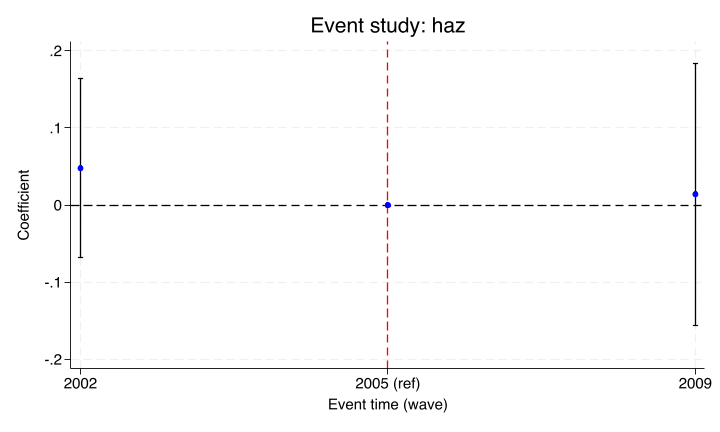
\includegraphics[width=0.8\textwidth]{event_study_haz.png}
\end{figure}

\begin{figure}[H]
\centering
\caption{Event Study, Weight-for-Age, Binary DID}
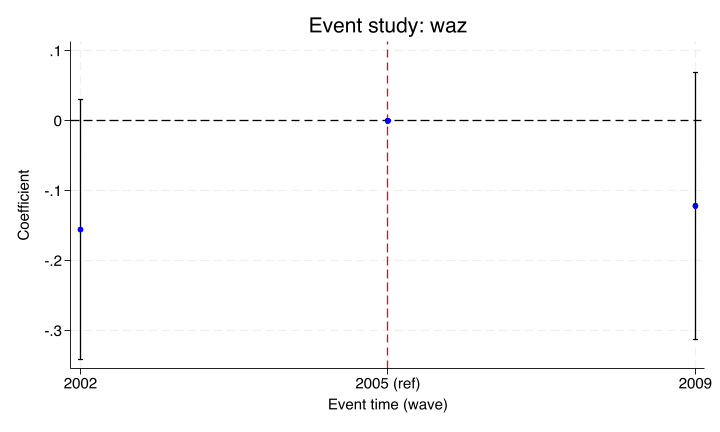
\includegraphics[width=0.8\textwidth]{event_study_waz.png}
\end{figure}

\begin{figure}[H]
\centering
\caption{Event Study, BMI-for-Age, Binary DID}
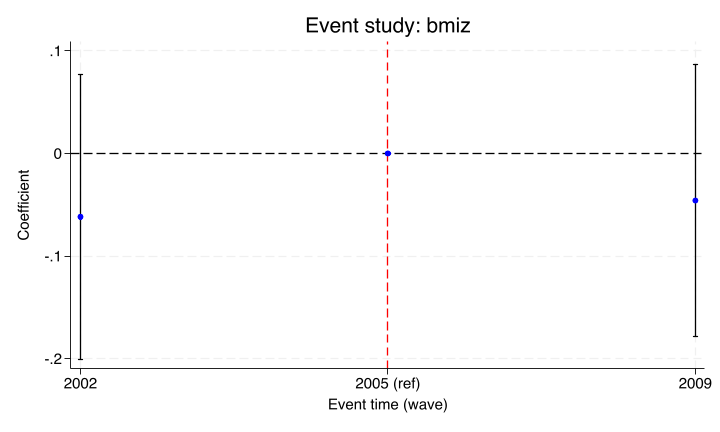
\includegraphics[width=0.8\textwidth]{event_study_bmiz.png}
\end{figure}

\begin{figure}[H]
\centering
\caption{Change in Height-for-Age by 2009 Rainfall Deficit, Continuous DID}
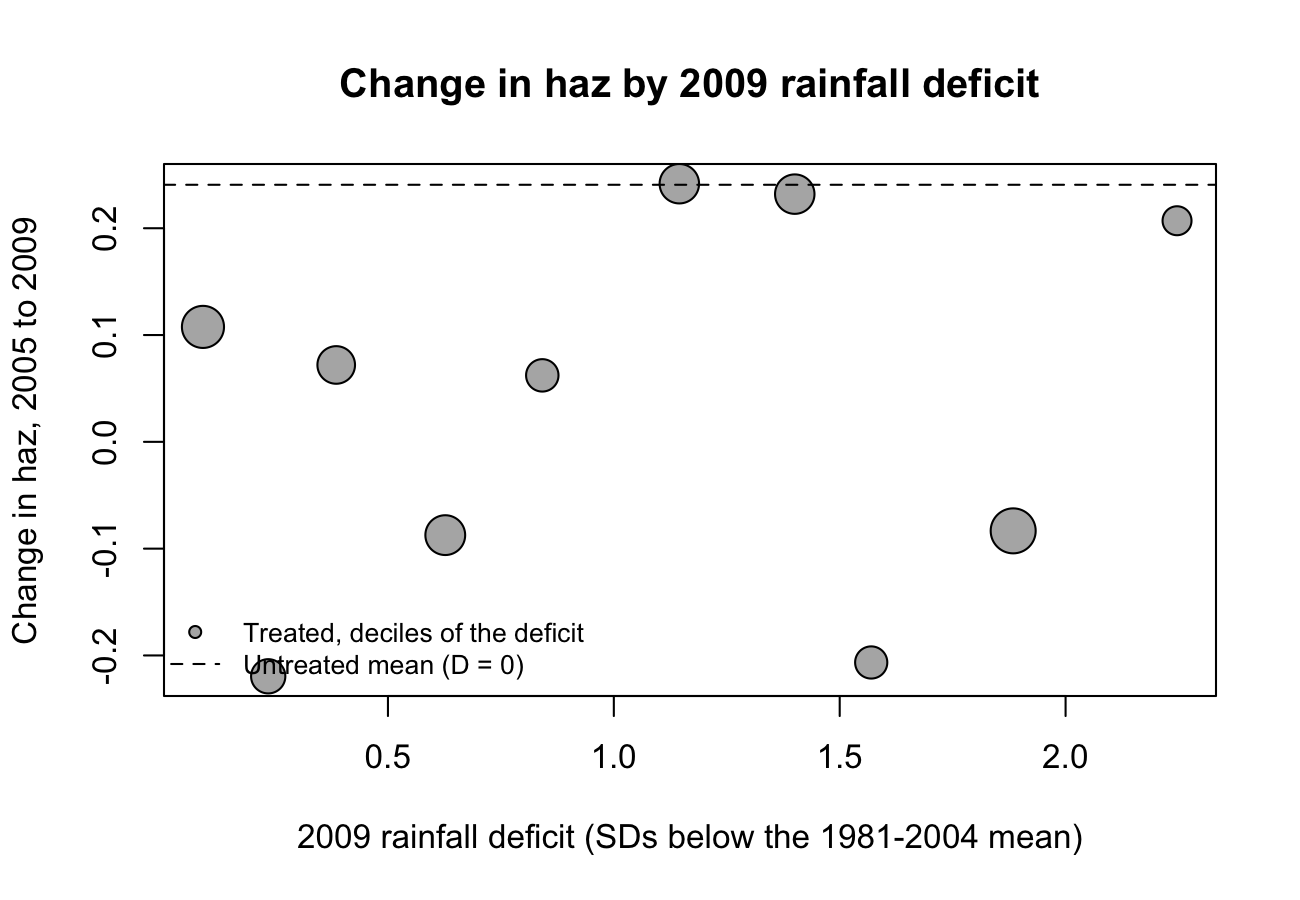
\includegraphics[width=0.8\textwidth]{contdid_binscatter_haz.png}
\end{figure}

\begin{figure}[H]
\centering
\caption{Change in Weight-for-Age by 2009 Rainfall Deficit, Continuous DID}
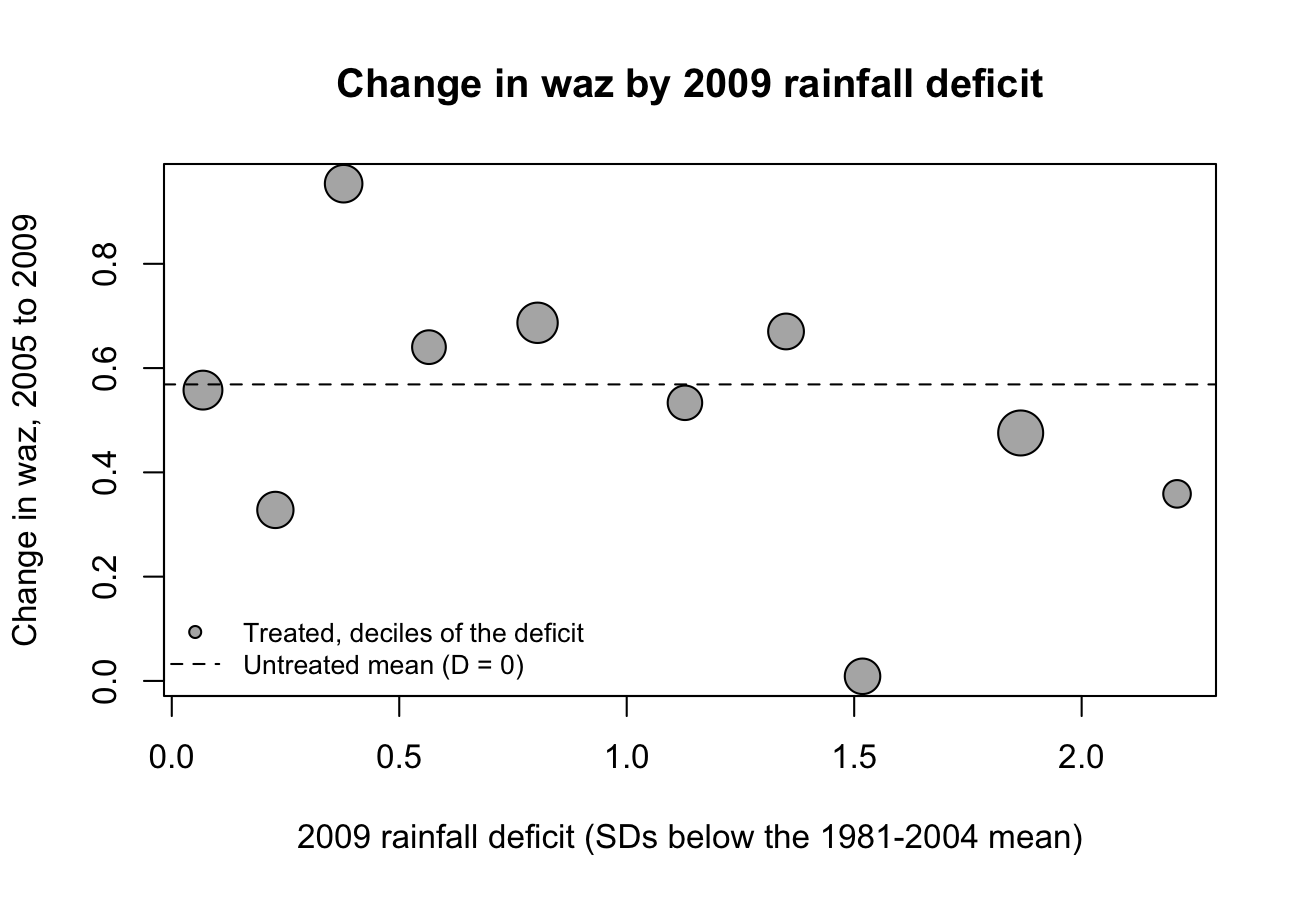
\includegraphics[width=0.8\textwidth]{contdid_binscatter_waz.png}
\end{figure}

\begin{figure}[H]
\centering
\caption{ATT by 2009 Rainfall Deficit, Height-for-Age, Continuous DID}
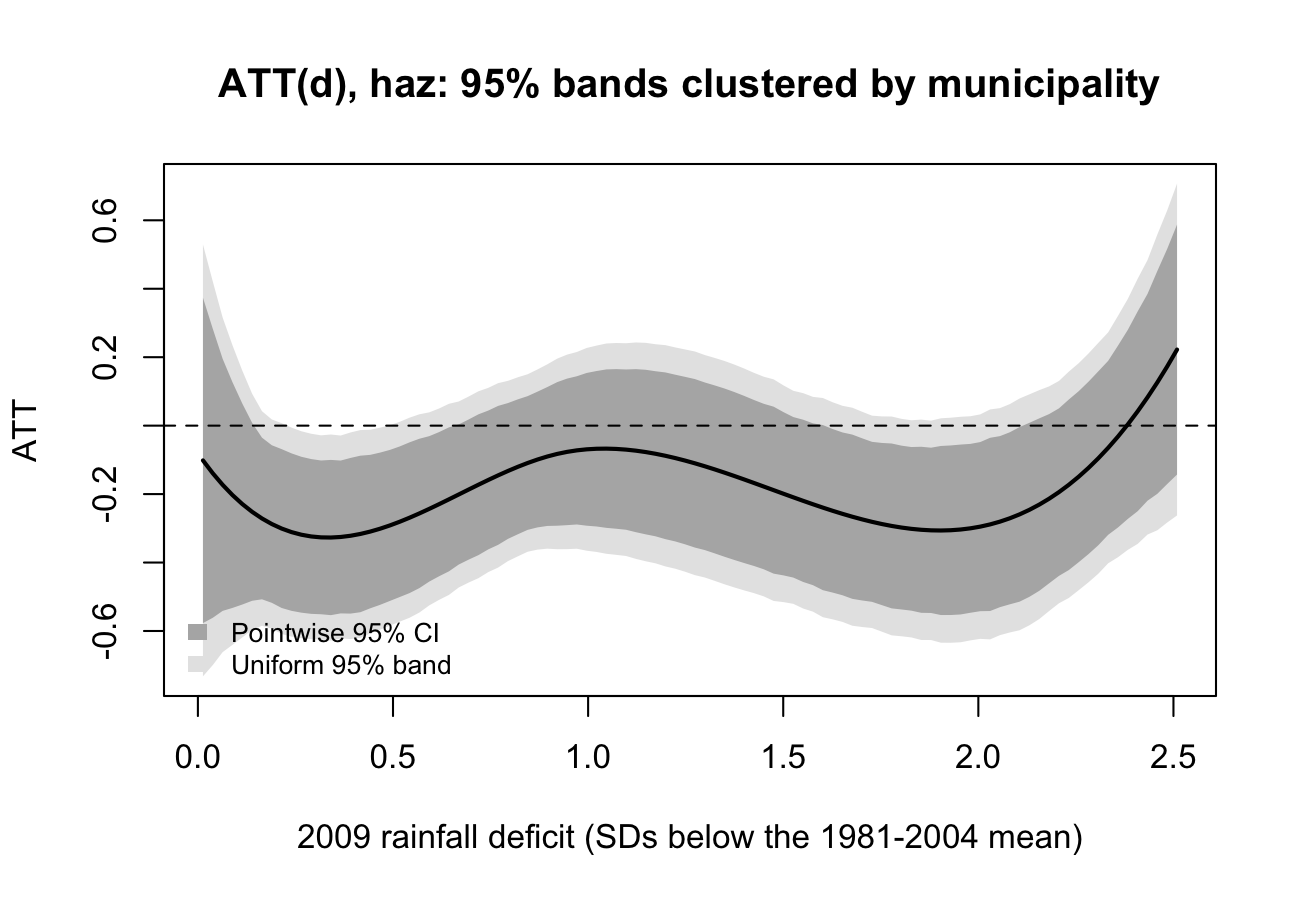
\includegraphics[width=0.8\textwidth]{contdid_att_clustered_haz.png}
\end{figure}

\clearpage
\section*{Appendix}

\begingroup
\footnotesize
\renewcommand{\arraystretch}{0.86}
\setlength{\tabcolsep}{4pt}
\setlength{\LTcapwidth}{\textwidth}
\begin{longtable}{l*{5}{c}}
\caption{2009 Drought and Height-for-Age, Binary DID, All Three Waves}\\
\toprule
 & \multicolumn{5}{c}{Height-for-age z-score (HAZ)}\\
\cmidrule(lr){2-6}
            &\multicolumn{1}{c}{(1)}         &\multicolumn{1}{c}{(2)}         &\multicolumn{1}{c}{(3)}         &\multicolumn{1}{c}{(4)}         &\multicolumn{1}{c}{(5)}         \\
\midrule
Drought \ensuremath{\times} post&       0.081         &       0.128         &       0.138         &       0.177         &       0.135         \\
            &     (0.085)         &     (0.089)         &     (0.095)         &     (0.148)         &     (0.100)         \\
Drought \ensuremath{\times} post \ensuremath{\times} 2002 remittances&                     &                     &                     &                     &      -0.127         \\
            &                     &                     &                     &                     &     (0.139)         \\
2002 remittances \ensuremath{\times} post&                     &                     &                     &                     &      -0.099         \\
            &                     &                     &                     &                     &     (0.094)         \\
\midrule
2005--2008 droughts \ensuremath{\times} post&           N         &           Y         &           Y         &           Y         &           Y         \\
2002 household controls \ensuremath{\times} post&           N         &           N         &           Y         &           Y         &           Y         \\
2005 child and mother controls \ensuremath{\times} post&           N         &           N         &           Y         &           Y         &           Y         \\
2005 father and birth controls \ensuremath{\times} post&           N         &           N         &           N         &           Y         &           N         \\
Child FE    &           Y         &           Y         &           Y         &           Y         &           Y         \\
Interview year-month FE&           Y         &           Y         &           Y         &           Y         &           Y         \\
Children    &       1,293         &       1,293         &       1,084         &         559         &       1,003         \\
\bottomrule
\addlinespace[6pt]\multicolumn{6}{p{0.97\textwidth}}{\scriptsize \textit{Notes:} This robustness check keeps only children measured in all three waves (2002, 2005 and 2009), so the event study pre-trend test and the 2005--2009 DID come from the same children, and changes in sample composition, such as attrition or children first measured in 2005, cannot drive the estimates. The table reports the effect of the 2009 drought on the WHO height-for-age z-score (HAZ) with the binary DID for these children, aged 15 or younger in both rounds, with a 2005 municipality and not measured in MxFLS-3 before November 2009.
Columns, variables and controls are as in the main binary DID tables. All regressions include child and interview year-month fixed effects, and standard errors are clustered by 2005 municipality. \sym{*}\(p<.10\), \sym{**}\(p<.05\), \sym{***}\(p<.01\).}\\
\end{longtable}
\endgroup
\clearpage
\begingroup
\footnotesize
\renewcommand{\arraystretch}{0.86}
\setlength{\tabcolsep}{4pt}
\setlength{\LTcapwidth}{\textwidth}
\begin{longtable}{l*{5}{c}}
\caption{2009 Drought and Weight-for-Age, Binary DID, All Three Waves}\\
\toprule
 & \multicolumn{5}{c}{Weight-for-age z-score (WAZ)}\\
\cmidrule(lr){2-6}
            &\multicolumn{1}{c}{(1)}         &\multicolumn{1}{c}{(2)}         &\multicolumn{1}{c}{(3)}         &\multicolumn{1}{c}{(4)}         &\multicolumn{1}{c}{(5)}         \\
\midrule
Drought \ensuremath{\times} post&       0.016         &      -0.068         &      -0.026         &      -0.078         &       0.166         \\
            &     (0.127)         &     (0.151)         &     (0.163)         &     (0.252)         &     (0.210)         \\
Drought \ensuremath{\times} post \ensuremath{\times} 2002 remittances&                     &                     &                     &                     &      -0.142         \\
            &                     &                     &                     &                     &     (0.383)         \\
2002 remittances \ensuremath{\times} post&                     &                     &                     &                     &       0.008         \\
            &                     &                     &                     &                     &     (0.273)         \\
\midrule
2005--2008 droughts \ensuremath{\times} post&           N         &           Y         &           Y         &           Y         &           Y         \\
2002 household controls \ensuremath{\times} post&           N         &           N         &           Y         &           Y         &           Y         \\
2005 child and mother controls \ensuremath{\times} post&           N         &           N         &           Y         &           Y         &           Y         \\
2005 father and birth controls \ensuremath{\times} post&           N         &           N         &           N         &           Y         &           N         \\
Child FE    &           Y         &           Y         &           Y         &           Y         &           Y         \\
Interview year-month FE&           Y         &           Y         &           Y         &           Y         &           Y         \\
Children    &         266         &         266         &         203         &         121         &         179         \\
\bottomrule
\addlinespace[6pt]\multicolumn{6}{p{0.97\textwidth}}{\scriptsize \textit{Notes:} This robustness check keeps only children measured in all three waves (2002, 2005 and 2009), so the event study pre-trend test and the 2005--2009 DID come from the same children, and changes in sample composition, such as attrition or children first measured in 2005, cannot drive the estimates. The table reports the effect of the 2009 drought on the WHO weight-for-age z-score (WAZ) with the binary DID for these children, aged 10 or younger in both rounds, with a 2005 municipality and not measured in MxFLS-3 before November 2009.
Columns, variables and controls are as in the main binary DID tables. All regressions include child and interview year-month fixed effects, and standard errors are clustered by 2005 municipality. \sym{*}\(p<.10\), \sym{**}\(p<.05\), \sym{***}\(p<.01\).}\\
\end{longtable}
\endgroup
\clearpage
\begingroup
\footnotesize
\renewcommand{\arraystretch}{0.86}
\setlength{\tabcolsep}{4pt}
\setlength{\LTcapwidth}{\textwidth}
\begin{longtable}{l*{5}{c}}
\caption{2009 Drought and BMI-for-Age, Binary DID, All Three Waves}\\
\toprule
 & \multicolumn{5}{c}{BMI-for-age z-score (BMIZ)}\\
\cmidrule(lr){2-6}
            &\multicolumn{1}{c}{(1)}         &\multicolumn{1}{c}{(2)}         &\multicolumn{1}{c}{(3)}         &\multicolumn{1}{c}{(4)}         &\multicolumn{1}{c}{(5)}         \\
\midrule
Drought \ensuremath{\times} post&      -0.038         &       0.006         &      -0.010         &      -0.069         &       0.044         \\
            &     (0.098)         &     (0.105)         &     (0.110)         &     (0.108)         &     (0.127)         \\
Drought \ensuremath{\times} post \ensuremath{\times} 2002 remittances&                     &                     &                     &                     &      -0.092         \\
            &                     &                     &                     &                     &     (0.235)         \\
2002 remittances \ensuremath{\times} post&                     &                     &                     &                     &       0.064         \\
            &                     &                     &                     &                     &     (0.087)         \\
\midrule
2005--2008 droughts \ensuremath{\times} post&           N         &           Y         &           Y         &           Y         &           Y         \\
2002 household controls \ensuremath{\times} post&           N         &           N         &           Y         &           Y         &           Y         \\
2005 child and mother controls \ensuremath{\times} post&           N         &           N         &           Y         &           Y         &           Y         \\
2005 father and birth controls \ensuremath{\times} post&           N         &           N         &           N         &           Y         &           N         \\
Child FE    &           Y         &           Y         &           Y         &           Y         &           Y         \\
Interview year-month FE&           Y         &           Y         &           Y         &           Y         &           Y         \\
Children    &       1,196         &       1,196         &       1,006         &         513         &         933         \\
\bottomrule
\addlinespace[6pt]\multicolumn{6}{p{0.97\textwidth}}{\scriptsize \textit{Notes:} This robustness check keeps only children measured in all three waves (2002, 2005 and 2009), so the event study pre-trend test and the 2005--2009 DID come from the same children, and changes in sample composition, such as attrition or children first measured in 2005, cannot drive the estimates. The table reports the effect of the 2009 drought on the WHO BMI-for-age z-score (BMIZ) with the binary DID for these children, aged 15 or younger in both rounds, with a 2005 municipality and not measured in MxFLS-3 before November 2009.
Columns, variables and controls are as in the main binary DID tables. All regressions include child and interview year-month fixed effects, and standard errors are clustered by 2005 municipality. \sym{*}\(p<.10\), \sym{**}\(p<.05\), \sym{***}\(p<.01\).}\\
\end{longtable}
\endgroup
\clearpage
\begingroup
\footnotesize
\renewcommand{\arraystretch}{0.86}
\setlength{\tabcolsep}{4pt}
\setlength{\LTcapwidth}{\textwidth}
\begin{longtable}{l*{5}{c}}
\caption{2009 Drought and Height-for-Age, Binary DID, Boys}\\
\toprule
 & \multicolumn{5}{c}{Height-for-age z-score (HAZ)}\\
\cmidrule(lr){2-6}
            &\multicolumn{1}{c}{(1)}         &\multicolumn{1}{c}{(2)}         &\multicolumn{1}{c}{(3)}         &\multicolumn{1}{c}{(4)}         &\multicolumn{1}{c}{(5)}         \\
\midrule
Drought \ensuremath{\times} post&      -0.020         &       0.066         &      -0.016         &       0.258         &      -0.032         \\
            &     (0.126)         &     (0.136)         &     (0.149)         &     (0.250)         &     (0.141)         \\
Drought \ensuremath{\times} post \ensuremath{\times} 2002 remittances&                     &                     &                     &                     &      -0.214         \\
            &                     &                     &                     &                     &     (0.233)         \\
2002 remittances \ensuremath{\times} post&                     &                     &                     &                     &      -0.273\sym{**} \\
            &                     &                     &                     &                     &     (0.130)         \\
\midrule
2005--2008 droughts \ensuremath{\times} post&           N         &           Y         &           Y         &           Y         &           Y         \\
2002 household controls \ensuremath{\times} post&           N         &           N         &           Y         &           Y         &           Y         \\
2005 child and mother controls \ensuremath{\times} post&           N         &           N         &           Y         &           Y         &           Y         \\
2005 father and birth controls \ensuremath{\times} post&           N         &           N         &           N         &           Y         &           N         \\
Child FE    &           Y         &           Y         &           Y         &           Y         &           Y         \\
Interview year-month FE&           Y         &           Y         &           Y         &           Y         &           Y         \\
Children    &       1,201         &       1,201         &         869         &         353         &         806         \\
\bottomrule
\addlinespace[6pt]\multicolumn{6}{p{0.97\textwidth}}{\scriptsize \textit{Notes:} Estimating the effect separately for boys and girls tests for gender disparities in the impact of the drought, as households facing an income shock may protect the nutrition and health of sons and daughters differently. The table reports the effect of the 2009 drought on the WHO height-for-age z-score (HAZ) with the binary DID for boys (2005 roster sex), aged 15 or younger in both rounds, with a 2005 municipality and not measured in MxFLS-3 before November 2009.
Columns, variables and controls are as in the main binary DID tables, without child sex in the controls. All regressions include child and interview year-month fixed effects, and standard errors are clustered by 2005 municipality. \sym{*}\(p<.10\), \sym{**}\(p<.05\), \sym{***}\(p<.01\).}\\
\end{longtable}
\endgroup
\clearpage
\begingroup
\footnotesize
\renewcommand{\arraystretch}{0.86}
\setlength{\tabcolsep}{4pt}
\setlength{\LTcapwidth}{\textwidth}
\begin{longtable}{l*{5}{c}}
\caption{2009 Drought and Weight-for-Age, Binary DID, Boys}\\
\toprule
 & \multicolumn{5}{c}{Weight-for-age z-score (WAZ)}\\
\cmidrule(lr){2-6}
            &\multicolumn{1}{c}{(1)}         &\multicolumn{1}{c}{(2)}         &\multicolumn{1}{c}{(3)}         &\multicolumn{1}{c}{(4)}         &\multicolumn{1}{c}{(5)}         \\
\midrule
Drought \ensuremath{\times} post&      -0.168         &      -0.125         &      -0.269         &      -0.426         &      -0.140         \\
            &     (0.149)         &     (0.161)         &     (0.182)         &     (0.326)         &     (0.212)         \\
Drought \ensuremath{\times} post \ensuremath{\times} 2002 remittances&                     &                     &                     &                     &      -0.022         \\
            &                     &                     &                     &                     &     (0.293)         \\
2002 remittances \ensuremath{\times} post&                     &                     &                     &                     &       0.008         \\
            &                     &                     &                     &                     &     (0.179)         \\
\midrule
2005--2008 droughts \ensuremath{\times} post&           N         &           Y         &           Y         &           Y         &           Y         \\
2002 household controls \ensuremath{\times} post&           N         &           N         &           Y         &           Y         &           Y         \\
2005 child and mother controls \ensuremath{\times} post&           N         &           N         &           Y         &           Y         &           Y         \\
2005 father and birth controls \ensuremath{\times} post&           N         &           N         &           N         &           Y         &           N         \\
Child FE    &           Y         &           Y         &           Y         &           Y         &           Y         \\
Interview year-month FE&           Y         &           Y         &           Y         &           Y         &           Y         \\
Children    &         551         &         551         &         367         &         103         &         331         \\
\bottomrule
\addlinespace[6pt]\multicolumn{6}{p{0.97\textwidth}}{\scriptsize \textit{Notes:} Estimating the effect separately for boys and girls tests for gender disparities in the impact of the drought, as households facing an income shock may protect the nutrition and health of sons and daughters differently. The table reports the effect of the 2009 drought on the WHO weight-for-age z-score (WAZ) with the binary DID for boys (2005 roster sex), aged 10 or younger in both rounds, with a 2005 municipality and not measured in MxFLS-3 before November 2009.
Columns, variables and controls are as in the main binary DID tables, without child sex in the controls. All regressions include child and interview year-month fixed effects, and standard errors are clustered by 2005 municipality. \sym{*}\(p<.10\), \sym{**}\(p<.05\), \sym{***}\(p<.01\).}\\
\end{longtable}
\endgroup
\clearpage
\begingroup
\footnotesize
\renewcommand{\arraystretch}{0.86}
\setlength{\tabcolsep}{4pt}
\setlength{\LTcapwidth}{\textwidth}
\begin{longtable}{l*{5}{c}}
\caption{2009 Drought and BMI-for-Age, Binary DID, Boys}\\
\toprule
 & \multicolumn{5}{c}{BMI-for-age z-score (BMIZ)}\\
\cmidrule(lr){2-6}
            &\multicolumn{1}{c}{(1)}         &\multicolumn{1}{c}{(2)}         &\multicolumn{1}{c}{(3)}         &\multicolumn{1}{c}{(4)}         &\multicolumn{1}{c}{(5)}         \\
\midrule
Drought \ensuremath{\times} post&      -0.160         &      -0.141         &      -0.214\sym{*}  &      -0.189         &      -0.332\sym{**} \\
            &     (0.101)         &     (0.103)         &     (0.116)         &     (0.149)         &     (0.150)         \\
Drought \ensuremath{\times} post \ensuremath{\times} 2002 remittances&                     &                     &                     &                     &       0.459         \\
            &                     &                     &                     &                     &     (0.298)         \\
2002 remittances \ensuremath{\times} post&                     &                     &                     &                     &      -0.083         \\
            &                     &                     &                     &                     &     (0.116)         \\
\midrule
2005--2008 droughts \ensuremath{\times} post&           N         &           Y         &           Y         &           Y         &           Y         \\
2002 household controls \ensuremath{\times} post&           N         &           N         &           Y         &           Y         &           Y         \\
2005 child and mother controls \ensuremath{\times} post&           N         &           N         &           Y         &           Y         &           Y         \\
2005 father and birth controls \ensuremath{\times} post&           N         &           N         &           N         &           Y         &           N         \\
Child FE    &           Y         &           Y         &           Y         &           Y         &           Y         \\
Interview year-month FE&           Y         &           Y         &           Y         &           Y         &           Y         \\
Children    &       1,170         &       1,170         &         847         &         346         &         787         \\
\bottomrule
\addlinespace[6pt]\multicolumn{6}{p{0.97\textwidth}}{\scriptsize \textit{Notes:} Estimating the effect separately for boys and girls tests for gender disparities in the impact of the drought, as households facing an income shock may protect the nutrition and health of sons and daughters differently. The table reports the effect of the 2009 drought on the WHO BMI-for-age z-score (BMIZ) with the binary DID for boys (2005 roster sex), aged 15 or younger in both rounds, with a 2005 municipality and not measured in MxFLS-3 before November 2009.
Columns, variables and controls are as in the main binary DID tables, without child sex in the controls. All regressions include child and interview year-month fixed effects, and standard errors are clustered by 2005 municipality. \sym{*}\(p<.10\), \sym{**}\(p<.05\), \sym{***}\(p<.01\).}\\
\end{longtable}
\endgroup
\clearpage
\begingroup
\footnotesize
\renewcommand{\arraystretch}{0.86}
\setlength{\tabcolsep}{4pt}
\setlength{\LTcapwidth}{\textwidth}
\begin{longtable}{l*{5}{c}}
\caption{2009 Drought and Height-for-Age, Binary DID, Girls}\\
\toprule
 & \multicolumn{5}{c}{Height-for-age z-score (HAZ)}\\
\cmidrule(lr){2-6}
            &\multicolumn{1}{c}{(1)}         &\multicolumn{1}{c}{(2)}         &\multicolumn{1}{c}{(3)}         &\multicolumn{1}{c}{(4)}         &\multicolumn{1}{c}{(5)}         \\
\midrule
Drought \ensuremath{\times} post&       0.007         &       0.015         &      -0.004         &       0.035         &      -0.085         \\
            &     (0.096)         &     (0.103)         &     (0.116)         &     (0.194)         &     (0.134)         \\
Drought \ensuremath{\times} post \ensuremath{\times} 2002 remittances&                     &                     &                     &                     &       0.002         \\
            &                     &                     &                     &                     &     (0.182)         \\
2002 remittances \ensuremath{\times} post&                     &                     &                     &                     &      -0.171         \\
            &                     &                     &                     &                     &     (0.122)         \\
\midrule
2005--2008 droughts \ensuremath{\times} post&           N         &           Y         &           Y         &           Y         &           Y         \\
2002 household controls \ensuremath{\times} post&           N         &           N         &           Y         &           Y         &           Y         \\
2005 child and mother controls \ensuremath{\times} post&           N         &           N         &           Y         &           Y         &           Y         \\
2005 father and birth controls \ensuremath{\times} post&           N         &           N         &           N         &           Y         &           N         \\
Child FE    &           Y         &           Y         &           Y         &           Y         &           Y         \\
Interview year-month FE&           Y         &           Y         &           Y         &           Y         &           Y         \\
Children    &       1,220         &       1,220         &         878         &         377         &         811         \\
\bottomrule
\addlinespace[6pt]\multicolumn{6}{p{0.97\textwidth}}{\scriptsize \textit{Notes:} Estimating the effect separately for boys and girls tests for gender disparities in the impact of the drought, as households facing an income shock may protect the nutrition and health of sons and daughters differently. The table reports the effect of the 2009 drought on the WHO height-for-age z-score (HAZ) with the binary DID for girls (2005 roster sex), aged 15 or younger in both rounds, with a 2005 municipality and not measured in MxFLS-3 before November 2009.
Columns, variables and controls are as in the main binary DID tables, without child sex in the controls. All regressions include child and interview year-month fixed effects, and standard errors are clustered by 2005 municipality. \sym{*}\(p<.10\), \sym{**}\(p<.05\), \sym{***}\(p<.01\).}\\
\end{longtable}
\endgroup
\clearpage
\begingroup
\footnotesize
\renewcommand{\arraystretch}{0.86}
\setlength{\tabcolsep}{4pt}
\setlength{\LTcapwidth}{\textwidth}
\begin{longtable}{l*{5}{c}}
\caption{2009 Drought and Weight-for-Age, Binary DID, Girls}\\
\toprule
 & \multicolumn{5}{c}{Weight-for-age z-score (WAZ)}\\
\cmidrule(lr){2-6}
            &\multicolumn{1}{c}{(1)}         &\multicolumn{1}{c}{(2)}         &\multicolumn{1}{c}{(3)}         &\multicolumn{1}{c}{(4)}         &\multicolumn{1}{c}{(5)}         \\
\midrule
Drought \ensuremath{\times} post&      -0.248\sym{**} &      -0.303\sym{**} &      -0.508\sym{***}&      -0.593\sym{*}  &      -0.507\sym{***}\\
            &     (0.107)         &     (0.116)         &     (0.137)         &     (0.316)         &     (0.170)         \\
Drought \ensuremath{\times} post \ensuremath{\times} 2002 remittances&                     &                     &                     &                     &      -0.316         \\
            &                     &                     &                     &                     &     (0.323)         \\
2002 remittances \ensuremath{\times} post&                     &                     &                     &                     &       0.056         \\
            &                     &                     &                     &                     &     (0.189)         \\
\midrule
2005--2008 droughts \ensuremath{\times} post&           N         &           Y         &           Y         &           Y         &           Y         \\
2002 household controls \ensuremath{\times} post&           N         &           N         &           Y         &           Y         &           Y         \\
2005 child and mother controls \ensuremath{\times} post&           N         &           N         &           Y         &           Y         &           Y         \\
2005 father and birth controls \ensuremath{\times} post&           N         &           N         &           N         &           Y         &           N         \\
Child FE    &           Y         &           Y         &           Y         &           Y         &           Y         \\
Interview year-month FE&           Y         &           Y         &           Y         &           Y         &           Y         \\
Children    &         520         &         520         &         324         &         115         &         295         \\
\bottomrule
\addlinespace[6pt]\multicolumn{6}{p{0.97\textwidth}}{\scriptsize \textit{Notes:} Estimating the effect separately for boys and girls tests for gender disparities in the impact of the drought, as households facing an income shock may protect the nutrition and health of sons and daughters differently. The table reports the effect of the 2009 drought on the WHO weight-for-age z-score (WAZ) with the binary DID for girls (2005 roster sex), aged 10 or younger in both rounds, with a 2005 municipality and not measured in MxFLS-3 before November 2009.
Columns, variables and controls are as in the main binary DID tables, without child sex in the controls. All regressions include child and interview year-month fixed effects, and standard errors are clustered by 2005 municipality. \sym{*}\(p<.10\), \sym{**}\(p<.05\), \sym{***}\(p<.01\).}\\
\end{longtable}
\endgroup
\clearpage
\begingroup
\footnotesize
\renewcommand{\arraystretch}{0.86}
\setlength{\tabcolsep}{4pt}
\setlength{\LTcapwidth}{\textwidth}
\begin{longtable}{l*{5}{c}}
\caption{2009 Drought and BMI-for-Age, Binary DID, Girls}\\
\toprule
 & \multicolumn{5}{c}{BMI-for-age z-score (BMIZ)}\\
\cmidrule(lr){2-6}
            &\multicolumn{1}{c}{(1)}         &\multicolumn{1}{c}{(2)}         &\multicolumn{1}{c}{(3)}         &\multicolumn{1}{c}{(4)}         &\multicolumn{1}{c}{(5)}         \\
\midrule
Drought \ensuremath{\times} post&      -0.076         &      -0.064         &      -0.151         &      -0.117         &      -0.000         \\
            &     (0.082)         &     (0.101)         &     (0.123)         &     (0.165)         &     (0.130)         \\
Drought \ensuremath{\times} post \ensuremath{\times} 2002 remittances&                     &                     &                     &                     &      -0.489\sym{**} \\
            &                     &                     &                     &                     &     (0.196)         \\
2002 remittances \ensuremath{\times} post&                     &                     &                     &                     &       0.133         \\
            &                     &                     &                     &                     &     (0.097)         \\
\midrule
2005--2008 droughts \ensuremath{\times} post&           N         &           Y         &           Y         &           Y         &           Y         \\
2002 household controls \ensuremath{\times} post&           N         &           N         &           Y         &           Y         &           Y         \\
2005 child and mother controls \ensuremath{\times} post&           N         &           N         &           Y         &           Y         &           Y         \\
2005 father and birth controls \ensuremath{\times} post&           N         &           N         &           N         &           Y         &           N         \\
Child FE    &           Y         &           Y         &           Y         &           Y         &           Y         \\
Interview year-month FE&           Y         &           Y         &           Y         &           Y         &           Y         \\
Children    &       1,199         &       1,199         &         861         &         364         &         795         \\
\bottomrule
\addlinespace[6pt]\multicolumn{6}{p{0.97\textwidth}}{\scriptsize \textit{Notes:} Estimating the effect separately for boys and girls tests for gender disparities in the impact of the drought, as households facing an income shock may protect the nutrition and health of sons and daughters differently. The table reports the effect of the 2009 drought on the WHO BMI-for-age z-score (BMIZ) with the binary DID for girls (2005 roster sex), aged 15 or younger in both rounds, with a 2005 municipality and not measured in MxFLS-3 before November 2009.
Columns, variables and controls are as in the main binary DID tables, without child sex in the controls. All regressions include child and interview year-month fixed effects, and standard errors are clustered by 2005 municipality. \sym{*}\(p<.10\), \sym{**}\(p<.05\), \sym{***}\(p<.01\).}\\
\end{longtable}
\endgroup
\clearpage
\begingroup
\footnotesize
\renewcommand{\arraystretch}{0.86}
\setlength{\tabcolsep}{4pt}
\setlength{\LTcapwidth}{\textwidth}
\begin{longtable}{l*{5}{c}}
\caption{2009 Drought and Height-for-Age, Binary DID, Rural Children}\\
\toprule
 & \multicolumn{5}{c}{Height-for-age z-score (HAZ)}\\
\cmidrule(lr){2-6}
            &\multicolumn{1}{c}{(1)}         &\multicolumn{1}{c}{(2)}         &\multicolumn{1}{c}{(3)}         &\multicolumn{1}{c}{(4)}         &\multicolumn{1}{c}{(5)}         \\
\midrule
Drought \ensuremath{\times} post&       0.079         &       0.342\sym{**} &       0.443\sym{***}&       0.640\sym{***}&       0.401\sym{**} \\
            &     (0.153)         &     (0.141)         &     (0.146)         &     (0.224)         &     (0.178)         \\
Drought \ensuremath{\times} post \ensuremath{\times} 2002 remittances&                     &                     &                     &                     &      -0.091         \\
            &                     &                     &                     &                     &     (0.278)         \\
2002 remittances \ensuremath{\times} post&                     &                     &                     &                     &      -0.084         \\
            &                     &                     &                     &                     &     (0.166)         \\
\midrule
2005--2008 droughts \ensuremath{\times} post&           N         &           Y         &           Y         &           Y         &           Y         \\
2002 household controls \ensuremath{\times} post&           N         &           N         &           Y         &           Y         &           Y         \\
2005 child and mother controls \ensuremath{\times} post&           N         &           N         &           Y         &           Y         &           Y         \\
2005 father and birth controls \ensuremath{\times} post&           N         &           N         &           N         &           Y         &           N         \\
Child FE    &           Y         &           Y         &           Y         &           Y         &           Y         \\
Interview year-month FE&           Y         &           Y         &           Y         &           Y         &           Y         \\
Children    &       1,016         &       1,016         &         732         &         272         &         714         \\
\bottomrule
\addlinespace[6pt]\multicolumn{6}{p{0.97\textwidth}}{\scriptsize \textit{Notes:} Estimating the effect separately for rural and urban children tests whether the drought hits harder where household incomes depend more directly on rain-fed agriculture, while urban households are mainly exposed through food prices. Rural is a locality with fewer than 2,500 inhabitants (INEGI, 2024). The table reports the effect of the 2009 drought on the WHO height-for-age z-score (HAZ) with the binary DID for rural children (2005 household locality), aged 15 or younger in both rounds, with a 2005 municipality and not measured in MxFLS-3 before November 2009.
Columns, variables and controls are as in the main binary DID tables, without rural in the controls. All regressions include child and interview year-month fixed effects, and standard errors are clustered by 2005 municipality. \sym{*}\(p<.10\), \sym{**}\(p<.05\), \sym{***}\(p<.01\).}\\
\end{longtable}
\endgroup
\clearpage
\begingroup
\footnotesize
\renewcommand{\arraystretch}{0.86}
\setlength{\tabcolsep}{4pt}
\setlength{\LTcapwidth}{\textwidth}
\begin{longtable}{l*{5}{c}}
\caption{2009 Drought and Weight-for-Age, Binary DID, Rural Children}\\
\toprule
 & \multicolumn{5}{c}{Weight-for-age z-score (WAZ)}\\
\cmidrule(lr){2-6}
            &\multicolumn{1}{c}{(1)}         &\multicolumn{1}{c}{(2)}         &\multicolumn{1}{c}{(3)}         &\multicolumn{1}{c}{(4)}         &\multicolumn{1}{c}{(5)}         \\
\midrule
Drought \ensuremath{\times} post&      -0.204         &      -0.068         &      -0.323         &      -0.457         &      -0.304         \\
            &     (0.157)         &     (0.161)         &     (0.252)         &     (0.417)         &     (0.268)         \\
Drought \ensuremath{\times} post \ensuremath{\times} 2002 remittances&                     &                     &                     &                     &      -0.151         \\
            &                     &                     &                     &                     &     (0.325)         \\
2002 remittances \ensuremath{\times} post&                     &                     &                     &                     &       0.108         \\
            &                     &                     &                     &                     &     (0.219)         \\
\midrule
2005--2008 droughts \ensuremath{\times} post&           N         &           Y         &           Y         &           Y         &           Y         \\
2002 household controls \ensuremath{\times} post&           N         &           N         &           Y         &           Y         &           Y         \\
2005 child and mother controls \ensuremath{\times} post&           N         &           N         &           Y         &           Y         &           Y         \\
2005 father and birth controls \ensuremath{\times} post&           N         &           N         &           N         &           Y         &           N         \\
Child FE    &           Y         &           Y         &           Y         &           Y         &           Y         \\
Interview year-month FE&           Y         &           Y         &           Y         &           Y         &           Y         \\
Children    &         414         &         414         &         265         &          85         &         260         \\
\bottomrule
\addlinespace[6pt]\multicolumn{6}{p{0.97\textwidth}}{\scriptsize \textit{Notes:} Estimating the effect separately for rural and urban children tests whether the drought hits harder where household incomes depend more directly on rain-fed agriculture, while urban households are mainly exposed through food prices. Rural is a locality with fewer than 2,500 inhabitants (INEGI, 2024). The table reports the effect of the 2009 drought on the WHO weight-for-age z-score (WAZ) with the binary DID for rural children (2005 household locality), aged 10 or younger in both rounds, with a 2005 municipality and not measured in MxFLS-3 before November 2009.
Columns, variables and controls are as in the main binary DID tables, without rural in the controls. All regressions include child and interview year-month fixed effects, and standard errors are clustered by 2005 municipality. \sym{*}\(p<.10\), \sym{**}\(p<.05\), \sym{***}\(p<.01\).}\\
\end{longtable}
\endgroup
\clearpage
\begingroup
\footnotesize
\renewcommand{\arraystretch}{0.86}
\setlength{\tabcolsep}{4pt}
\setlength{\LTcapwidth}{\textwidth}
\begin{longtable}{l*{5}{c}}
\caption{2009 Drought and BMI-for-Age, Binary DID, Rural Children}\\
\toprule
 & \multicolumn{5}{c}{BMI-for-age z-score (BMIZ)}\\
\cmidrule(lr){2-6}
            &\multicolumn{1}{c}{(1)}         &\multicolumn{1}{c}{(2)}         &\multicolumn{1}{c}{(3)}         &\multicolumn{1}{c}{(4)}         &\multicolumn{1}{c}{(5)}         \\
\midrule
Drought \ensuremath{\times} post&      -0.054         &      -0.028         &      -0.154         &      -0.227         &      -0.137         \\
            &     (0.113)         &     (0.144)         &     (0.175)         &     (0.221)         &     (0.197)         \\
Drought \ensuremath{\times} post \ensuremath{\times} 2002 remittances&                     &                     &                     &                     &      -0.052         \\
            &                     &                     &                     &                     &     (0.259)         \\
2002 remittances \ensuremath{\times} post&                     &                     &                     &                     &       0.097         \\
            &                     &                     &                     &                     &     (0.113)         \\
\midrule
2005--2008 droughts \ensuremath{\times} post&           N         &           Y         &           Y         &           Y         &           Y         \\
2002 household controls \ensuremath{\times} post&           N         &           N         &           Y         &           Y         &           Y         \\
2005 child and mother controls \ensuremath{\times} post&           N         &           N         &           Y         &           Y         &           Y         \\
2005 father and birth controls \ensuremath{\times} post&           N         &           N         &           N         &           Y         &           N         \\
Child FE    &           Y         &           Y         &           Y         &           Y         &           Y         \\
Interview year-month FE&           Y         &           Y         &           Y         &           Y         &           Y         \\
Children    &         998         &         998         &         719         &         264         &         701         \\
\bottomrule
\addlinespace[6pt]\multicolumn{6}{p{0.97\textwidth}}{\scriptsize \textit{Notes:} Estimating the effect separately for rural and urban children tests whether the drought hits harder where household incomes depend more directly on rain-fed agriculture, while urban households are mainly exposed through food prices. Rural is a locality with fewer than 2,500 inhabitants (INEGI, 2024). The table reports the effect of the 2009 drought on the WHO BMI-for-age z-score (BMIZ) with the binary DID for rural children (2005 household locality), aged 15 or younger in both rounds, with a 2005 municipality and not measured in MxFLS-3 before November 2009.
Columns, variables and controls are as in the main binary DID tables, without rural in the controls. All regressions include child and interview year-month fixed effects, and standard errors are clustered by 2005 municipality. \sym{*}\(p<.10\), \sym{**}\(p<.05\), \sym{***}\(p<.01\).}\\
\end{longtable}
\endgroup
\clearpage
\begingroup
\footnotesize
\renewcommand{\arraystretch}{0.86}
\setlength{\tabcolsep}{4pt}
\setlength{\LTcapwidth}{\textwidth}
\begin{longtable}{l*{5}{c}}
\caption{2009 Drought and Height-for-Age, Binary DID, Urban Children}\\
\toprule
 & \multicolumn{5}{c}{Height-for-age z-score (HAZ)}\\
\cmidrule(lr){2-6}
            &\multicolumn{1}{c}{(1)}         &\multicolumn{1}{c}{(2)}         &\multicolumn{1}{c}{(3)}         &\multicolumn{1}{c}{(4)}         &\multicolumn{1}{c}{(5)}         \\
\midrule
Drought \ensuremath{\times} post&      -0.108         &      -0.186         &      -0.277\sym{**} &      -0.302         &      -0.327\sym{**} \\
            &     (0.110)         &     (0.130)         &     (0.127)         &     (0.197)         &     (0.140)         \\
Drought \ensuremath{\times} post \ensuremath{\times} 2002 remittances&                     &                     &                     &                     &      -0.018         \\
            &                     &                     &                     &                     &     (0.179)         \\
2002 remittances \ensuremath{\times} post&                     &                     &                     &                     &      -0.321\sym{**} \\
            &                     &                     &                     &                     &     (0.127)         \\
\midrule
2005--2008 droughts \ensuremath{\times} post&           N         &           Y         &           Y         &           Y         &           Y         \\
2002 household controls \ensuremath{\times} post&           N         &           N         &           Y         &           Y         &           Y         \\
2005 child and mother controls \ensuremath{\times} post&           N         &           N         &           Y         &           Y         &           Y         \\
2005 father and birth controls \ensuremath{\times} post&           N         &           N         &           N         &           Y         &           N         \\
Child FE    &           Y         &           Y         &           Y         &           Y         &           Y         \\
Interview year-month FE&           Y         &           Y         &           Y         &           Y         &           Y         \\
Children    &       1,412         &       1,412         &       1,020         &         455         &         904         \\
\bottomrule
\addlinespace[6pt]\multicolumn{6}{p{0.97\textwidth}}{\scriptsize \textit{Notes:} Estimating the effect separately for rural and urban children tests whether the drought hits harder where household incomes depend more directly on rain-fed agriculture, while urban households are mainly exposed through food prices. Rural is a locality with fewer than 2,500 inhabitants (INEGI, 2024). The table reports the effect of the 2009 drought on the WHO height-for-age z-score (HAZ) with the binary DID for urban children (2005 household locality), aged 15 or younger in both rounds, with a 2005 municipality and not measured in MxFLS-3 before November 2009.
Columns, variables and controls are as in the main binary DID tables, without rural in the controls. All regressions include child and interview year-month fixed effects, and standard errors are clustered by 2005 municipality. \sym{*}\(p<.10\), \sym{**}\(p<.05\), \sym{***}\(p<.01\).}\\
\end{longtable}
\endgroup
\clearpage
\begingroup
\footnotesize
\renewcommand{\arraystretch}{0.86}
\setlength{\tabcolsep}{4pt}
\setlength{\LTcapwidth}{\textwidth}
\begin{longtable}{l*{5}{c}}
\caption{2009 Drought and Weight-for-Age, Binary DID, Urban Children}\\
\toprule
 & \multicolumn{5}{c}{Weight-for-age z-score (WAZ)}\\
\cmidrule(lr){2-6}
            &\multicolumn{1}{c}{(1)}         &\multicolumn{1}{c}{(2)}         &\multicolumn{1}{c}{(3)}         &\multicolumn{1}{c}{(4)}         &\multicolumn{1}{c}{(5)}         \\
\midrule
Drought \ensuremath{\times} post&      -0.200         &      -0.351\sym{**} &      -0.508\sym{***}&      -0.385         &      -0.400\sym{**} \\
            &     (0.127)         &     (0.138)         &     (0.142)         &     (0.288)         &     (0.159)         \\
Drought \ensuremath{\times} post \ensuremath{\times} 2002 remittances&                     &                     &                     &                     &      -0.401         \\
            &                     &                     &                     &                     &     (0.259)         \\
2002 remittances \ensuremath{\times} post&                     &                     &                     &                     &       0.013         \\
            &                     &                     &                     &                     &     (0.138)         \\
\midrule
2005--2008 droughts \ensuremath{\times} post&           N         &           Y         &           Y         &           Y         &           Y         \\
2002 household controls \ensuremath{\times} post&           N         &           N         &           Y         &           Y         &           Y         \\
2005 child and mother controls \ensuremath{\times} post&           N         &           N         &           Y         &           Y         &           Y         \\
2005 father and birth controls \ensuremath{\times} post&           N         &           N         &           N         &           Y         &           N         \\
Child FE    &           Y         &           Y         &           Y         &           Y         &           Y         \\
Interview year-month FE&           Y         &           Y         &           Y         &           Y         &           Y         \\
Children    &         654         &         654         &         427         &         137         &         365         \\
\bottomrule
\addlinespace[6pt]\multicolumn{6}{p{0.97\textwidth}}{\scriptsize \textit{Notes:} Estimating the effect separately for rural and urban children tests whether the drought hits harder where household incomes depend more directly on rain-fed agriculture, while urban households are mainly exposed through food prices. Rural is a locality with fewer than 2,500 inhabitants (INEGI, 2024). The table reports the effect of the 2009 drought on the WHO weight-for-age z-score (WAZ) with the binary DID for urban children (2005 household locality), aged 10 or younger in both rounds, with a 2005 municipality and not measured in MxFLS-3 before November 2009.
Columns, variables and controls are as in the main binary DID tables, without rural in the controls. All regressions include child and interview year-month fixed effects, and standard errors are clustered by 2005 municipality. \sym{*}\(p<.10\), \sym{**}\(p<.05\), \sym{***}\(p<.01\).}\\
\end{longtable}
\endgroup
\clearpage
\begingroup
\footnotesize
\renewcommand{\arraystretch}{0.86}
\setlength{\tabcolsep}{4pt}
\setlength{\LTcapwidth}{\textwidth}
\begin{longtable}{l*{5}{c}}
\caption{2009 Drought and BMI-for-Age, Binary DID, Urban Children}\\
\toprule
 & \multicolumn{5}{c}{BMI-for-age z-score (BMIZ)}\\
\cmidrule(lr){2-6}
            &\multicolumn{1}{c}{(1)}         &\multicolumn{1}{c}{(2)}         &\multicolumn{1}{c}{(3)}         &\multicolumn{1}{c}{(4)}         &\multicolumn{1}{c}{(5)}         \\
\midrule
Drought \ensuremath{\times} post&      -0.144\sym{*}  &      -0.130         &      -0.208\sym{**} &      -0.006         &      -0.197         \\
            &     (0.081)         &     (0.087)         &     (0.100)         &     (0.141)         &     (0.126)         \\
Drought \ensuremath{\times} post \ensuremath{\times} 2002 remittances&                     &                     &                     &                     &       0.021         \\
            &                     &                     &                     &                     &     (0.314)         \\
2002 remittances \ensuremath{\times} post&                     &                     &                     &                     &       0.053         \\
            &                     &                     &                     &                     &     (0.109)         \\
\midrule
2005--2008 droughts \ensuremath{\times} post&           N         &           Y         &           Y         &           Y         &           Y         \\
2002 household controls \ensuremath{\times} post&           N         &           N         &           Y         &           Y         &           Y         \\
2005 child and mother controls \ensuremath{\times} post&           N         &           N         &           Y         &           Y         &           Y         \\
2005 father and birth controls \ensuremath{\times} post&           N         &           N         &           N         &           Y         &           N         \\
Child FE    &           Y         &           Y         &           Y         &           Y         &           Y         \\
Interview year-month FE&           Y         &           Y         &           Y         &           Y         &           Y         \\
Children    &       1,377         &       1,377         &         992         &         441         &         882         \\
\bottomrule
\addlinespace[6pt]\multicolumn{6}{p{0.97\textwidth}}{\scriptsize \textit{Notes:} Estimating the effect separately for rural and urban children tests whether the drought hits harder where household incomes depend more directly on rain-fed agriculture, while urban households are mainly exposed through food prices. Rural is a locality with fewer than 2,500 inhabitants (INEGI, 2024). The table reports the effect of the 2009 drought on the WHO BMI-for-age z-score (BMIZ) with the binary DID for urban children (2005 household locality), aged 15 or younger in both rounds, with a 2005 municipality and not measured in MxFLS-3 before November 2009.
Columns, variables and controls are as in the main binary DID tables, without rural in the controls. All regressions include child and interview year-month fixed effects, and standard errors are clustered by 2005 municipality. \sym{*}\(p<.10\), \sym{**}\(p<.05\), \sym{***}\(p<.01\).}\\
\end{longtable}
\endgroup
\clearpage
\begingroup
\footnotesize
\renewcommand{\arraystretch}{0.86}
\setlength{\tabcolsep}{4pt}
\setlength{\LTcapwidth}{\textwidth}
\begin{longtable}{l*{2}{c}}
\caption{Event Study, 2009 Drought and Height-for-Age}\\
\toprule
 & \multicolumn{2}{c}{Height-for-age z-score (HAZ)}\\
\cmidrule(lr){2-3}
            &\multicolumn{1}{c}{(1)}&\multicolumn{1}{c}{(2)}\\
            &\multicolumn{1}{c}{Event study}&\multicolumn{1}{c}{Triple difference}\\
\midrule
Drought \ensuremath{\times} 2002 wave (lead)&       0.048         &       0.050         \\
            &     (0.059)         &     (0.071)         \\
Drought \ensuremath{\times} 2009 wave&       0.014         &      -0.085         \\
            &     (0.087)         &     (0.101)         \\
Drought \ensuremath{\times} 2002 remittances \ensuremath{\times} 2002 wave (lead)&                     &      -0.082         \\
            &                     &     (0.112)         \\
Drought \ensuremath{\times} 2002 remittances \ensuremath{\times} 2009 wave&                     &      -0.026         \\
            &                     &     (0.129)         \\
\midrule
Child FE    &           Y         &           Y         \\
Interview year-month FE&           Y         &           Y         \\
P-value, lead = 0&       0.422         &       0.464         \\
\midrule 2009 drought effect, remittance households&                     &      -0.110         \\
\quad SE    &                     &       0.136         \\
\quad P-value&                     &       0.419         \\
\midrule Observations (child-waves)&      10,399         &       8,518         \\
Children    &       4,550         &       3,690         \\
2005 municipalities (clusters)&         143         &         136         \\
\bottomrule
\addlinespace[6pt]\multicolumn{3}{p{0.97\textwidth}}{\scriptsize \textit{Notes:} This table tests for pre-trends before the 2009 drought. Regressions are at the child-wave level and use MxFLS-1 (2002), MxFLS-2 (2005) and MxFLS-3 (2009), with 2005 as the
reference wave. The sample is children aged 15 or younger in each wave they are in, with a 2005 municipality, and not measured in MxFLS-3 before November 2009. Col. 1 regresses the outcome on the drought times the 2002 wave (the lead) and times the 2009
wave. Col. 2 adds the same terms times 2002 remittances, and the 2002 remittance terms on their own (not shown), for children with 2002 remittances observed. The P-value of the lead tests the drought lead in Col. 1 and the triple difference lead in Col. 2.
The effect for remittance households is the sum of the two 2009 drought terms. All regressions include child and interview year-month fixed effects, and standard errors are clustered by 2005 municipality. \sym{*}\(p<.10\), \sym{**}\(p<.05\), \sym{***}\(p<.01\).}\\
\end{longtable}
\endgroup
\clearpage
\begingroup
\footnotesize
\renewcommand{\arraystretch}{0.86}
\setlength{\tabcolsep}{4pt}
\setlength{\LTcapwidth}{\textwidth}
\begin{longtable}{l*{2}{c}}
\caption{Event Study, 2009 Drought and Weight-for-Age}\\
\toprule
 & \multicolumn{2}{c}{Weight-for-age z-score (WAZ)}\\
\cmidrule(lr){2-3}
            &\multicolumn{1}{c}{(1)}&\multicolumn{1}{c}{(2)}\\
            &\multicolumn{1}{c}{Event study}&\multicolumn{1}{c}{Triple difference}\\
\midrule
Drought \ensuremath{\times} 2002 wave (lead)&      -0.156         &      -0.063         \\
            &     (0.095)         &     (0.100)         \\
Drought \ensuremath{\times} 2009 wave&      -0.122         &      -0.160         \\
            &     (0.097)         &     (0.139)         \\
Drought \ensuremath{\times} 2002 remittances \ensuremath{\times} 2002 wave (lead)&                     &      -0.303\sym{*}  \\
            &                     &     (0.157)         \\
Drought \ensuremath{\times} 2002 remittances \ensuremath{\times} 2009 wave&                     &      -0.113         \\
            &                     &     (0.186)         \\
\midrule
Child FE    &           Y         &           Y         \\
Interview year-month FE&           Y         &           Y         \\
P-value, lead = 0&       0.103         &       0.056         \\
\midrule 2009 drought effect, remittance households&                     &      -0.273         \\
\quad SE    &                     &       0.160         \\
\quad P-value&                     &       0.090         \\
\midrule Observations (child-waves)&       4,959         &       3,848         \\
Children    &       2,342         &       1,817         \\
2005 municipalities (clusters)&         137         &         127         \\
\bottomrule
\addlinespace[6pt]\multicolumn{3}{p{0.97\textwidth}}{\scriptsize \textit{Notes:} This table tests for pre-trends before the 2009 drought. Regressions are at the child-wave level and use MxFLS-1 (2002), MxFLS-2 (2005) and MxFLS-3 (2009), with 2005 as the
reference wave. The sample is children aged 10 or younger in each wave they are in, with a 2005 municipality, and not measured in MxFLS-3 before November 2009. Col. 1 regresses the outcome on the drought times the 2002 wave (the lead) and times the 2009
wave. Col. 2 adds the same terms times 2002 remittances, and the 2002 remittance terms on their own (not shown), for children with 2002 remittances observed. The P-value of the lead tests the drought lead in Col. 1 and the triple difference lead in Col. 2.
The effect for remittance households is the sum of the two 2009 drought terms. All regressions include child and interview year-month fixed effects, and standard errors are clustered by 2005 municipality. \sym{*}\(p<.10\), \sym{**}\(p<.05\), \sym{***}\(p<.01\).}\\
\end{longtable}
\endgroup
\clearpage
\begingroup
\footnotesize
\renewcommand{\arraystretch}{0.86}
\setlength{\tabcolsep}{4pt}
\setlength{\LTcapwidth}{\textwidth}
\begin{longtable}{l*{2}{c}}
\caption{Event Study, 2009 Drought and BMI-for-Age}\\
\toprule
 & \multicolumn{2}{c}{BMI-for-age z-score (BMIZ)}\\
\cmidrule(lr){2-3}
            &\multicolumn{1}{c}{(1)}&\multicolumn{1}{c}{(2)}\\
            &\multicolumn{1}{c}{Event study}&\multicolumn{1}{c}{Triple difference}\\
\midrule
Drought \ensuremath{\times} 2002 wave (lead)&      -0.062         &      -0.054         \\
            &     (0.071)         &     (0.088)         \\
Drought \ensuremath{\times} 2009 wave&      -0.046         &      -0.075         \\
            &     (0.068)         &     (0.099)         \\
Drought \ensuremath{\times} 2002 remittances \ensuremath{\times} 2002 wave (lead)&                     &      -0.004         \\
            &                     &     (0.129)         \\
Drought \ensuremath{\times} 2002 remittances \ensuremath{\times} 2009 wave&                     &       0.061         \\
            &                     &     (0.192)         \\
\midrule
Child FE    &           Y         &           Y         \\
Interview year-month FE&           Y         &           Y         \\
P-value, lead = 0&       0.385         &       0.973         \\
\midrule 2009 drought effect, remittance households&                     &      -0.014         \\
\quad SE    &                     &       0.142         \\
\quad P-value&                     &       0.922         \\
\midrule Observations (child-waves)&       9,978         &       8,163         \\
Children    &       4,388         &       3,554         \\
2005 municipalities (clusters)&         143         &         136         \\
\bottomrule
\addlinespace[6pt]\multicolumn{3}{p{0.97\textwidth}}{\scriptsize \textit{Notes:} This table tests for pre-trends before the 2009 drought. Regressions are at the child-wave level and use MxFLS-1 (2002), MxFLS-2 (2005) and MxFLS-3 (2009), with 2005 as the
reference wave. The sample is children aged 15 or younger in each wave they are in, with a 2005 municipality, and not measured in MxFLS-3 before November 2009. Col. 1 regresses the outcome on the drought times the 2002 wave (the lead) and times the 2009
wave. Col. 2 adds the same terms times 2002 remittances, and the 2002 remittance terms on their own (not shown), for children with 2002 remittances observed. The P-value of the lead tests the drought lead in Col. 1 and the triple difference lead in Col. 2.
The effect for remittance households is the sum of the two 2009 drought terms. All regressions include child and interview year-month fixed effects, and standard errors are clustered by 2005 municipality. \sym{*}\(p<.10\), \sym{**}\(p<.05\), \sym{***}\(p<.01\).}\\
\end{longtable}
\endgroup
\clearpage
\begingroup
\footnotesize
\renewcommand{\arraystretch}{0.86}
\setlength{\tabcolsep}{4pt}
\setlength{\LTcapwidth}{\textwidth}
\begin{longtable}{l*{4}{c}}
\caption{Continuous DID by Subgroup, Height-for-Age}\\
\toprule
 & \multicolumn{4}{c}{Change in the height-for-age z-score (HAZ)}\\
\cmidrule(lr){2-5}
 & Boys & Girls & Rural & Urban\\
 & (1) & (2) & (3) & (4)\\
\midrule
Any 2009 deficit & -0.178 & -0.234\sym{**} & 0.086 & -0.288\sym{***}\\
 & (0.112) & (0.107) & (0.192) & (0.085)\\
 & [0.132] & [0.036] & [0.659] & [0.007]\\
Dry vs near normal, \ensuremath{z\le -1} & -0.005 & -0.004 & 0.170 & -0.118\\
 & (0.113) & (0.112) & (0.177) & (0.103)\\
 & [0.965] & [0.972] & [0.390] & [0.289]\\
Severely dry or worse vs near normal, \ensuremath{z\le -1.5} & -0.179 & -0.120 & 0.003 & -0.243\sym{*}\\
 & (0.151) & (0.127) & (0.257) & (0.112)\\
 & [0.278] & [0.410] & [0.992] & [0.057]\\
Dry \ensuremath{\times} 2002 remittances & -0.278 & 0.119 & -0.155 & -0.099\\
 & (0.222) & (0.173) & (0.227) & (0.168)\\
 & [0.225] & [0.506] & [0.506] & [0.564]\\
\midrule Children & 1,208 & 1,228 & 1,020 & 1,416\\
Municipalities with no 2009 deficit & 30 & 30 & 16 & 20\\
\bottomrule
\addlinespace[6pt]\multicolumn{5}{p{0.97\textwidth}}{\scriptsize \textit{Notes:} This table repeats the continuous DID and SPI results for the WHO height-for-age z-score (HAZ) by subgroup. Cols. 1--2 test for gender disparities in the impact of the drought (2005 roster sex),
and Cols. 3--4 test whether it hits rural children harder, as rural household incomes depend more directly on rain-fed agriculture. Rural is a locality with fewer than 2,500 inhabitants (INEGI, 2024). Rows, samples (aged 15 or younger in both rounds) and definitions are as in the main continuous DID and SPI
tables, and subgroups with few dry or untreated municipalities give noisy estimates. Standard errors clustered by 2005 municipality are in parentheses. Wild cluster bootstrap p-values are in brackets, which tend to be conservative with few treated municipalities (MacKinnon et al., 2023). Stars use the clustered p-values, and where a wild bootstrap p-value is shown both must pass: \sym{*}\(p<.10\), \sym{**}\(p<.05\), \sym{***}\(p<.01\).}\\
\end{longtable}
\endgroup
\clearpage
\begingroup
\footnotesize
\renewcommand{\arraystretch}{0.86}
\setlength{\tabcolsep}{4pt}
\setlength{\LTcapwidth}{\textwidth}
\begin{longtable}{l*{4}{c}}
\caption{Continuous DID by Subgroup, Weight-for-Age}\\
\toprule
 & \multicolumn{4}{c}{Change in the weight-for-age z-score (WAZ)}\\
\cmidrule(lr){2-5}
 & Boys & Girls & Rural & Urban\\
 & (1) & (2) & (3) & (4)\\
\midrule
Any 2009 deficit & -0.064 & -0.019 & 0.015 & 0.016\\
 & (0.155) & (0.108) & (0.243) & (0.090)\\
 & [0.692] & [0.855] & [0.952] & [0.861]\\
Dry vs near normal, \ensuremath{z\le -1} & -0.212 & -0.210\sym{*} & -0.133 & -0.224\sym{**}\\
 & (0.170) & (0.107) & (0.209) & (0.104)\\
 & [0.241] & [0.058] & [0.612] & [0.043]\\
Severely dry or worse vs near normal, \ensuremath{z\le -1.5} & -0.416 & -0.217 & -0.381 & -0.262\sym{*}\\
 & (0.244) & (0.163) & (0.311) & (0.139)\\
 & [0.128] & [0.235] & [0.456] & [0.099]\\
Dry \ensuremath{\times} 2002 remittances & 0.063 & -0.309 & 0.084 & -0.411\\
 & (0.298) & (0.275) & (0.346) & (0.245)\\
 & [0.842] & [0.263] & [0.825] & [0.100]\\
\midrule Children & 556 & 528 & 424 & 660\\
Municipalities with no 2009 deficit & 26 & 23 & 12 & 19\\
\bottomrule
\addlinespace[6pt]\multicolumn{5}{p{0.97\textwidth}}{\scriptsize \textit{Notes:} This table repeats the continuous DID and SPI results for the WHO weight-for-age z-score (WAZ) by subgroup. Cols. 1--2 test for gender disparities in the impact of the drought (2005 roster sex),
and Cols. 3--4 test whether it hits rural children harder, as rural household incomes depend more directly on rain-fed agriculture. Rural is a locality with fewer than 2,500 inhabitants (INEGI, 2024). Rows, samples (aged 10 or younger in both rounds) and definitions are as in the main continuous DID and SPI
tables, and subgroups with few dry or untreated municipalities give noisy estimates. Standard errors clustered by 2005 municipality are in parentheses. Wild cluster bootstrap p-values are in brackets, which tend to be conservative with few treated municipalities (MacKinnon et al., 2023). Stars use the clustered p-values, and where a wild bootstrap p-value is shown both must pass: \sym{*}\(p<.10\), \sym{**}\(p<.05\), \sym{***}\(p<.01\).}\\
\end{longtable}
\endgroup
\clearpage
\begingroup
\footnotesize
\renewcommand{\arraystretch}{0.86}
\setlength{\tabcolsep}{4pt}
\setlength{\LTcapwidth}{\textwidth}
\begin{longtable}{l*{4}{c}}
\caption{Continuous DID by Subgroup, BMI-for-Age}\\
\toprule
 & \multicolumn{4}{c}{Change in the BMI-for-age z-score (BMIZ)}\\
\cmidrule(lr){2-5}
 & Boys & Girls & Rural & Urban\\
 & (1) & (2) & (3) & (4)\\
\midrule
Any 2009 deficit & -0.009 & -0.043 & 0.023 & -0.049\\
 & (0.115) & (0.090) & (0.120) & (0.103)\\
 & [0.935] & [0.670] & [0.858] & [0.651]\\
Dry vs near normal, \ensuremath{z\le -1} & -0.171 & -0.085 & -0.085 & -0.160\\
 & (0.101) & (0.081) & (0.102) & (0.107)\\
 & [0.105] & [0.309] & [0.439] & [0.170]\\
Severely dry or worse vs near normal, \ensuremath{z\le -1.5} & -0.144 & -0.114 & -0.190 & -0.087\\
 & (0.100) & (0.090) & (0.099) & (0.079)\\
 & [0.171] & [0.239] & [0.125] & [0.292]\\
Dry \ensuremath{\times} 2002 remittances & 0.541 & -0.388\sym{**} & 0.058 & 0.065\\
 & (0.308) & (0.169) & (0.241) & (0.295)\\
 & [0.107] & [0.030] & [0.824] & [0.842]\\
\midrule Children & 1,177 & 1,206 & 1,002 & 1,381\\
Municipalities with no 2009 deficit & 30 & 30 & 16 & 20\\
\bottomrule
\addlinespace[6pt]\multicolumn{5}{p{0.97\textwidth}}{\scriptsize \textit{Notes:} This table repeats the continuous DID and SPI results for the WHO BMI-for-age z-score (BMIZ) by subgroup. Cols. 1--2 test for gender disparities in the impact of the drought (2005 roster sex),
and Cols. 3--4 test whether it hits rural children harder, as rural household incomes depend more directly on rain-fed agriculture. Rural is a locality with fewer than 2,500 inhabitants (INEGI, 2024). Rows, samples (aged 15 or younger in both rounds) and definitions are as in the main continuous DID and SPI
tables, and subgroups with few dry or untreated municipalities give noisy estimates. Standard errors clustered by 2005 municipality are in parentheses. Wild cluster bootstrap p-values are in brackets, which tend to be conservative with few treated municipalities (MacKinnon et al., 2023). Stars use the clustered p-values, and where a wild bootstrap p-value is shown both must pass: \sym{*}\(p<.10\), \sym{**}\(p<.05\), \sym{***}\(p<.01\).}\\
\end{longtable}
\endgroup

\end{document}
